% ============================================================
%  第二章 声子（§1–§10 + 章末参考文献）
%  底本：高等教育出版社《固体理论》（第二版）印刷页 18–61（PDF p038–p081）
%  OCR 输入：MinerU/full_merged.md 行 1142–3226
%  公式编号自检：§1 (2.1.1)–(2.1.27)；§2 (2.2.1)–(2.2.34)；
%    §3 (2.3.1)–(2.3.13)；§4 (2.4.1)–(2.4.24)；§5 (2.5.1)–(2.5.31)；
%    §6 (2.6.1)–(2.6.28)；§7 (2.7.1)–(2.7.17)；§8 (2.8.1)–(2.8.22)；
%    §9 (2.9.1)–(2.9.29)；§10 (2.10.1)–(2.10.34)。
%    共 259 个自动编号（OCR 有 258 个 tag：(2.2.25) 内容被 OCR 漏失，
%    按原书 p046 补排；(2.4.2) OCR tag 残缺为 {4.2}，原书 p052 有此式，
%    自动编号复原）。逐一对上，无跳号。
%  已修正的 OCR/原书错误：
%  1. 章首段"振动—晶格振动"按原书 p038 补全破折号为"振动——晶格振动"
%  2. (2.1.1) OCR 误作 X_l(t)=\dot R_l+u_l(t)，原书 p038 为 R_l（无点）
%  3. (2.1.3) 第二个求和下标 OCR 误作 l,β，原书为 l',β；(2.1.8) 同此（r→l'）
%  4. (2.1.10) OCR 漏下标：e^{ik·R}→e^{ik·R_l}
%  5. 行内"是沿 α(α=x,y,z) 方向的位移分量"OCR 乱码按原书 p038 复原
%  6. "由于式(2.1.6)并考虑到势能Φ为实函数……反演对称性后"OCR 串入
%     \barΦ/Φ 乱码，按原书 p040 复原
%  7. (2.1.20)–(2.1.24) 复式晶格诸式 OCR 乱码严重，按原书 p041 以
%     \binom{k}{s,s'} 记法复原；(2.1.26)/(2.1.27) 附近 M_s 错位同此
%  8. "构成3r维空间的本征矢量X_σ"OCR 漏 X_σ，按原书 p042 补
%  9. (2.2.3)/(2.2.4) 求和指标 n_l→R_l，首行指数 e^{-ik·R_l}→e^{-iαk·R_l}，
%     第二行 e^{-ik·e^{-1}R_l}→e^{-ik·α^{-1}R_l}（原书 p042）
% 10. "与传播方向方平行"原书 p046 排印衍一"方"字，删
% 11. "则本方征方程式(2.2.8)变为"原书 p043 排印错误，"本方征"→"本征"
% 12. (2.2.25) 原书为极化矢量式（p046），OCR 只剩编号，已按原书补排；
%     (2.2.24) 的频率两行原书共用一号，按原书排为一号
% 13. (2.2.22) OCR 拆成两个 $$ 块（ω₁² 行无号），原书共用 (2.2.22)，
%     按原书合并；(2.2.28)/(2.2.31)/(2.2.34) 同类处理
% 14. (2.2.29)/(2.2.30) OCR 矩阵/根式乱码，按原书 p048 复原
% 15. "例如二维正方晶格的 ω_σ(k) 和 e_{kσ} 的计算……计算准至第二近邻"
%     及"其中 f_l=f₁(l=1,2,3,4), f_l=f₂(l=5,6,7,8)"OCR 乱码按原书 p044 复原
% 16. "有两支频谱 ω_±²(k)，其中由于 ω₋(k=0)=0……而 ω₊ 则代表光频支格波"
%     OCR 丢 ω₋/ω₊ 下标，按原书 p049 复原
% 17. §3 脚注①（"也可以约定 e_{kσ}=−e_{−kσ}，则 Q*_{kσ}=−Q_{−kσ}，其结果
%     相同."）整段被 OCR 漏失，按原书 p049 页脚补录
% 18. (2.3.11) OCR 作 e_{kα}^α，原书 p051 为 e_{kσ}^{α*}；(2.3.13) 同此
% 19. (2.4.2) OCR tag 残缺为 {4.2}；且原书 p052 两处极化矢量漏印共轭星号
%     （无星号则中间步推不出 δ_σσ'），按物理补 e_{kσ}^{α*}
% 20. (2.4.11) OCR 作 \tilde{=}，原书 p053 为等号
% 21. (2.4.15) 之后 ε'_n=nℏω 一行 OCR 漏"(n=1,2,3,⋯)"，按原书 p054 补
% 22. §4 末段"和动量 ℏk 的玻色粒子"OCR 误作"动量kk"；"|{n_{kσ}}>"态
%     记号乱码按原书 p056 复原
% 23. §5 "引入一个在空间缓变的位移场"OCR 误作"引人"；"u 就是 l 元胞中
%     质心的位移"OCR 误作"μ 就是"；均按原书 p056 改
% 24. §5 "只可能有 ∇·u、∇u 及 ∇×u 三种一阶导数"OCR 乱码（∇μ、串入
%     u(r)），按原书 p057 复原；"把晶体当作弹性各向同性体"OCR 串入 φ(r)，删
% 25. (2.5.8) 第二行漏 Σ_{μ,ν}，按原书 p057 补
% 26. "当然，严格的作法应从 ℒ=𝒯−φ 的拉格朗日方程导出"OCR 乱码按原书 p058 复原
% 27. (2.5.24) 第二行 OCR 作 ρ(r)，原书 p059 为动量场 p(r)；"它等于 Q̇*_{kσ}"
%     及"约定关系式(2.3.3)和(2.3.4)保持不变"OCR 错位按原书复原
% 28. "再作变换，引入声子的产生及消灭算符"OCR 串入 \vec{p}，删（原书 p059）
% 29. §5 脚注①（体积相对变化 Δ=δV/V=∇·u 推导）被 OCR 误置于 §6 正文，
%     按原书 p060 页脚归位为脚注；OCR 之 δ̃V、∂u^s/∂x 等乱码同此复原
% 30. §6 "M_± 为正、负离子的质量"OCR 漏下标 ±；"电荷量相等、符号相反的
%     离子"OCR 串入 \barπ，均按原书 p060 复原
% 31. (2.6.4)–(2.6.8) 的下标"弹性/极化"OCR 乱码，按原书 p061 复原为
%     \text{弹性}/\text{极化}
% 32. "(如高、低频介电常数 ε_∞、ε_0 等)"OCR 乱码按原书 p062 复原；
%     (2.6.16) 末尾 OCR 多一逗号，删
% 33. §7 首段"光子波数 k=ω/c=ω_T/c"OCR 误作"k:ω/c=…"；ω_±(k) 的 ±
%     下标多处脱落（含 (2.7.6) 前后特征 (i)(ii)(iii) 段），按原书 p064–p066 复原
% 34. §7 特征段"对于大 k 值"OCR 误作"大 h 值"；"ω₋类光及 ω₊类声"按原书复原
% 35. 图 2.8/2.9/2.10 三图原书并排于 p066，图注照录；OCR 之一幅无注图按
%     原书归位（裁剪图 hash 重复不影响占位排版）
% 36. (2.8.8) 求导下标 OCR 作"\_"，按原书 p068 补 V
% 37. (2.8.13) 第二行积分上限 OCR 作 ∞，原书 p069 为 ω_M
% 38. §8–§9 \underline{ĝ}、δ̂、\widehat\otimes 等噪声统一为 g、δ
% 39. "算出的态密集为"原书 p074 排印错误，"态密集"→"态密度"
% 40. §10 "影响. 从一维原子链入手"OCR 逗号按原书 p075 改句号；
%     (2.10.6) 整式乱码按原书 p076 复原为 u_l=(1/√N)Σ_k ξ_k e^{-ikla}
% 41. (2.10.12) OCR 串入 \pounds_k，按原书 p077 改回 ξ_k
% 42. §10 "式(2.10.14)的解相对于 ω_k 都朝高频方向略有移动"OCR 漏下标 k，
%     按原书 p077 补；"分立能级——局域模"破折号按原书 p081 补全
% 43. 其余：全角句点"．"→"."；删除 OCR 间隔符"~"；\mathrm{d} 收紧；
%     \pmb→\boldsymbol；§4/§7/§8 标题字间空格收紧
%  遗留问题：图 2.1–2.13 均为占位图（fig2-N.pdf），宽度按原书目测配置；
%  图 2.11 四联小图的 (a)–(d) 子图注含于占位图，未另排
% ============================================================
\chapter{声子}

\section{晶格动力学}

本节用经典力学方法讨论完整晶体中原子（离子）绕平衡位置的振动——晶格振动.为简单起见，先讨论每个元胞中只含一个原子(离子)的简单晶格情况，然后推广到含多个原子的复式晶格情况.

设晶体的元胞数为$N$，原子质量为$M$.晶体中第$l$个元胞中原子的平衡位置由正格矢$\boldsymbol{R}_l$描述，$\boldsymbol{u}_l$则代表此原子的位移.因此，在$t$时刻$l$元胞中原子的瞬时位置为
\begin{equation}
  \boldsymbol{X}_l(t)=\boldsymbol{R}_l+\boldsymbol{u}_l(t)\,,\quad
  \boldsymbol{R}_l=\sum_{i=1}^{3}l_i\boldsymbol{a}_i
\end{equation}
晶格振动的总动能
\begin{equation}
  T=\frac{1}{2}\sum_{l,\alpha}M\dot{u}_l^{\alpha}\dot{u}_l^{\alpha}
  \qquad(\alpha=x,y,z)
\end{equation}
这里$u_l^{\alpha}$是沿$\alpha\,(\alpha=x,y,z)$方向的位移分量.由于晶体中原子(离子)的运动限于微振动，其总势能可按$u_l^{\alpha}$展开表示
\begin{equation}
  \Phi=\Phi_0+\sum_{l,\alpha}\Phi_{\alpha}(l)u_l^{\alpha}
  +\frac{1}{2}\sum_{l,\alpha}\sum_{l',\beta}\Phi_{\alpha\beta}(l,l')u_l^{\alpha}u_{l'}^{\beta}+\cdots
\end{equation}
这里$\Phi_0$为一常数，代表晶体中所有原子都处于平衡位置时的势能，它对于晶格振动不起作用，而
\begin{equation}
  \Phi_{\alpha}(l)=\left(\frac{\partial\Phi}{\partial u_l^{\alpha}}\right)_0=0
\end{equation}
是由于在平衡点晶体的势能极小，其中下标0代表平衡点，宗量内的符号$l$是正格矢$\boldsymbol{R}_l$的缩写.$\Phi_{\alpha\beta}(l,l')$为二次导数
\begin{equation}
  \Phi_{\alpha\beta}(l,l')=\left(\frac{\partial^2\Phi}
  {\partial u_l^{\alpha}\partial u_{l'}^{\beta}}\right)_0
  =\Phi_{\beta\alpha}(l',l)
\end{equation}
其中最后一个等式来源于二次导数的对称性.当采用周期性边界条件时，晶体具有平移不变性，$\Phi_{\alpha\beta}(l,l')$只是$(\boldsymbol{R}_l-\boldsymbol{R}_{l'})$的函数.计入平移对称性后，上式可写为
\begin{equation}
  \Phi_{\alpha\beta}(l,l')=\Phi_{\alpha\beta}(l-l')=\Phi_{\beta\alpha}(l'-l)
\end{equation}
$\Phi_{\alpha\beta}(l-l')$代表$l'$元胞中原子沿$\beta$方向位移单位距离时对$l$元胞中原子作用力沿$\alpha$方向的分量，称为力常数，并有下列重要关系：
\begin{equation}
  \sum_{l'}\Phi_{\alpha\beta}(l-l')=0
\end{equation}
因为当整体作刚性位移(即每个原子均作$u_l^{\alpha}=v_{\alpha}$的位移)时，晶格中任一原子受到其它原子作用力之总和为零，即
\begin{equation*}
\begin{aligned}
  F_{\alpha}(l)&=-\frac{\partial\Phi}{\partial u^{\alpha}}
  =-\sum_{l',\beta}\Phi_{\alpha\beta}(l-l')u_{l'}^{\beta}\\
  &=-\sum_{\beta}\Bigl\{\sum_{l'}\Phi_{\alpha\beta}(l-l')\Bigr\}v_{\beta}=0
\end{aligned}
\end{equation*}
由于刚性位移量$v_{\beta}$可取任意值，因此上式中$\{\cdots\}=0$，此即关系式(2.1.7).

在简谐近似下，略去$\Phi$按位移$u$展开的三次方项，定义$\Delta\Phi=\Phi-\Phi_0$，则系统的振动哈密顿量为
\begin{equation}
  H=T+\Delta\Phi=\frac{1}{2M}\sum_{l,\alpha}p_l^{\alpha}p_l^{\alpha}
  +\frac{1}{2}\sum_{l,\alpha}\sum_{l',\beta}\Phi_{\alpha\beta}(l-l')u_l^{\alpha}u_{l'}^{\beta}
\end{equation}
其中$p_l^{\alpha}=M\dot{u}_l^{\alpha}$是$u_l^{\alpha}$的共轭力学量.系统的运动方程由经典力学的正则方程$\dot{p}_l^{\alpha}=-(\partial H/\partial u_l^{\alpha})$导出
\begin{equation}
  M\ddot{u}_l^{\alpha}=-\sum_{l',\beta}\Phi_{\alpha\beta}(l-l')u_{l'}^{\beta}
\end{equation}
其中利用了对称关系式(2.1.6).式(2.1.9)是$3N$个自由度的线性耦合振动方程组.利用平移对称性可使求解大为简化.将布洛赫定理，式(1.3.9)，用于晶格振动$u_l^{\alpha}$，应有
\begin{equation}
  u_l^{\alpha}=\mathrm{e}^{\mathrm{i}\boldsymbol{k}\cdot\boldsymbol{R}_l}u_0^{\alpha}
\end{equation}
对于每一确定$\boldsymbol{k}$值，运动方程的解表现出下列特性：

(i)各元胞中原子振动的方向相同，振幅相等；

(ii)有特定的相位关系，按$\mathrm{e}^{\mathrm{i}\boldsymbol{k}\cdot\boldsymbol{R}_l}$变化.

因此，每一确定$\boldsymbol{k}$的解代表波长为$\frac{2\pi}{|\boldsymbol{k}|}$的集体振动，称为格波.对于每一个$\boldsymbol{k}$，可确定方程式(2.1.9)的一个特解
\begin{equation*}
  \mathrm{e}^{\mathrm{i}\boldsymbol{k}\cdot\boldsymbol{R}_l}U_{\boldsymbol{k}}^{\alpha}
\end{equation*}
这里，令$u_0^{\alpha}=U_{\boldsymbol{k}}^{\alpha}$对应于用波矢$\boldsymbol{k}$标记的特解，将它代入式(2.1.9)，可将$3N$自由度的耦合方程组简化为$N$个独立的3自由度耦合方程组，而每个波矢满足方程：
\begin{equation}
  \ddot{U}_{\boldsymbol{k}}^{\alpha}=-\sum_{\beta}D_{\alpha\beta}(\boldsymbol{k})U_{\boldsymbol{k}}^{\beta}
  \quad(\alpha,\beta=x,y,z)
\end{equation}
其中
\begin{equation}
  D_{\alpha\beta}(\boldsymbol{k})\equiv\frac{1}{M}\sum_{l}\Phi_{\alpha\beta}(\boldsymbol{l})
  \mathrm{e}^{-\mathrm{i}\boldsymbol{k}\cdot\boldsymbol{R}_l}
\end{equation}
组成$3\times3$矩阵，代表力常数$\Phi$的傅里叶变换称为动力矩阵.由于式(2.1.6)并考虑到势能$\Phi$为实函数，易知，对于简单晶格考虑反演对称性后，$D_{\alpha\beta}(\boldsymbol{k})$应为实的厄米矩阵，其对角化方程(又称动力矩阵的本征方程)为
\begin{equation}
  \sum_{\beta}D_{\alpha\beta}(\boldsymbol{k})e_{\boldsymbol{k}}^{\beta}
  =\omega^2e_{\boldsymbol{k}}^{\alpha}
\end{equation}
这里，当$\omega$理解为振动频率时，$\omega^2$取正实量，具体由久期方程决定
\begin{equation}
  \det\parallel D_{\alpha\beta}(\boldsymbol{k})-\omega^2\delta_{\alpha\beta}\parallel=0
\end{equation}
可求出3个本征值
\begin{equation}
  \omega=\omega_{\sigma}(\boldsymbol{k})\qquad(\sigma=1,2,3)
\end{equation}
以及相应的3个实本征向量$\boldsymbol{e}_{\boldsymbol{k}\sigma}$，它们是描述各元胞中原子振动方向的单位矢，并满足下列正交性和完备性条件：
\begin{equation}
  \boldsymbol{e}_{\boldsymbol{k}\sigma}\cdot\boldsymbol{e}_{\boldsymbol{k}\sigma'}=\delta_{\sigma\sigma'}
\end{equation}
\begin{equation}
  \sum_{\sigma}e_{\boldsymbol{k}\sigma}^{\alpha}e_{\boldsymbol{k}\sigma}^{\beta}=\delta_{\alpha\beta}
\end{equation}
显然，利用式(2.1.13)可将运动方程式(2.1.11)退耦，并求出$U_{\boldsymbol{k}}^{\alpha}$正比于$e_{\boldsymbol{k}}^{\alpha}\mathrm{e}^{-\mathrm{i}\omega t}$的解.代入式(2.1.10)，有形式为
\begin{equation*}
  u_l^{\alpha}\sim\frac{1}{\sqrt{N}}e_{\boldsymbol{k}}^{\alpha}
  \mathrm{e}^{\mathrm{i}[\boldsymbol{k}\cdot\boldsymbol{R}_l-\omega t]}
\end{equation*}
的特解，其中$N$为元胞数，上式中若代入本征方程的解$\omega_{\sigma}(\boldsymbol{k})$和$\boldsymbol{e}_{\boldsymbol{k}\sigma}$就构成波矢$\boldsymbol{k}$，偏振$\sigma$，以及频率$\omega_{\sigma}(\boldsymbol{k})$的格波解.在BZ中，一定时刻$t$的格波解$N^{-\frac{1}{2}}e_{\boldsymbol{k}\sigma}^{\alpha}\mathrm{e}^{\mathrm{i}\boldsymbol{k}\cdot\boldsymbol{R}_l}$称为简正模，其中的相位因子仅仅来源于点阵的周期性.

根据正格矢与倒格矢间关系式(1.1.8)，立刻得到
\begin{equation}
  D_{\alpha\beta}(\boldsymbol{k}+\boldsymbol{K}_n)=D_{\alpha\beta}(\boldsymbol{k})
\end{equation}
动力矩阵是倒易点阵的周期函数，我们只需要在$\boldsymbol{k}$空间一个BZ内讨论，这里有$N$个不同的$\boldsymbol{k}$值，每一$\boldsymbol{k}$值又对应有3个本征值，共$3N$个简正模(或格波特解).根据式(1.3.16)、式(1.3.17)和式(2.1.16)、式(2.1.17)，这$3N$个简正模满足正交、归一和完备性条件，它们构成$3N$维空间的完备函数组，可用作基函数展开，表示$3N$自由度的晶格振动一般解：
\begin{equation}
  u_l^{\alpha}=\frac{1}{\sqrt{NM}}\sum_{\boldsymbol{k},\sigma}
  e_{\boldsymbol{k}\sigma}^{\alpha}Q_{\boldsymbol{k}\sigma}
  \mathrm{e}^{\mathrm{i}\boldsymbol{k}\cdot\boldsymbol{R}_l}
\end{equation}
系数$Q_{\boldsymbol{k}\sigma}$[包括$\mathrm{e}^{-\mathrm{i}\omega_{\sigma}(\boldsymbol{k})t}$因子]在固体物理学中称为简正坐标.$\boldsymbol{e}_{\boldsymbol{k}\sigma}$代表格波的偏振方向，通常称为极化矢量，它是单位矢.

方程式(2.1.11)对于各个不同的$\boldsymbol{k}$是彼此独立的，将它与式(2.1.9)相比较可知，原来的求解$3N$个线性联立方程已简化为$N$个独立$3\times3$矩阵$D(\boldsymbol{k})$的对角化问题，这是平移对称性起重要作用的例证.

对于元胞中有$r$个原子的复式晶格，动力矩阵的本征方程可直接由式(2.1.13)推广
\begin{equation}
  \sum_{\beta,s'}D_{\alpha\beta}\binom{\boldsymbol{k}}{s,s'}\,
  e_{\boldsymbol{k}}^{\beta}(s')=\omega^2e_{\boldsymbol{k}}^{\alpha}(s)
\end{equation}
其中$s$，$s'=1$，$\cdots$，$r$，代表元胞中不同的原子.格波频率由式(2.1.20)的系数行列式等于零决定
\begin{equation}
  \det\left\|\,D_{\alpha\beta}\binom{\boldsymbol{k}}{s,s'}
  -\omega^2\delta_{\alpha\beta}\delta_{ss'}\,\right\|=0
\end{equation}
它涉及$(3r\times3r)$矩阵对角化.其中动力矩阵取
\begin{equation}
  D_{\alpha\beta}\binom{\boldsymbol{k}}{s,s'}
  =\frac{1}{\sqrt{M_sM_{s'}}}\sum_{l}\Phi_{\alpha\beta}\binom{\boldsymbol{l}}{s,s'}
  \mathrm{e}^{-\mathrm{i}\boldsymbol{k}\cdot\boldsymbol{R}_l}
\end{equation}
可保证其厄米性.在复式晶格中，动力矩阵一般为复矩阵，仅在$\boldsymbol{k}=0$点(即$\Gamma$点)才简化为实矩阵.因此，除$\Gamma$点上的极化矢量为实矢量以外，其它点的极化矢量均为复量.力常数则由式(2.1.5)推广为
\begin{equation}
  \Phi_{\alpha\beta}\binom{l-l'}{s,s'}\equiv
  \left(\frac{\partial^2\Phi}{\partial u_l^{\alpha}(s)\,
  \partial u_{l'}^{\beta}(s')}\right)_0
\end{equation}
$u_l^{\alpha}(s)$代表$l$元胞中第$s$个原子在$\alpha$方向上的振动位移分量.与式(2.1.7)相对应，复式晶格中也有刚性位移不产生应力的重要关系：
\begin{equation}
  \sum_{l',s'}\Phi_{\alpha\beta}\binom{l-l'}{s,s'}=0
\end{equation}
本征方程式(2.1.20)决定$3r$个频率本征值
\begin{equation}
  \omega=\omega_{\sigma}(\boldsymbol{k})\qquad(\sigma=1,\cdots,3r)
\end{equation}
和相应的$3r$个复极化矢量$\boldsymbol{e}_{\boldsymbol{k}\sigma}(s)$.因此，复式晶格$l$元胞中第$s$个原子的位移为
\begin{equation}
  \boldsymbol{u}_l(s)=\frac{1}{\sqrt{NM_s}}\sum_{\boldsymbol{k},\sigma}
  \boldsymbol{e}_{\boldsymbol{k}\sigma}(s)Q_{\boldsymbol{k}\sigma}
  \mathrm{e}^{\mathrm{i}\boldsymbol{k}\cdot\boldsymbol{R}_l}
\end{equation}
其中相位因子反映点阵周期性，$M_s$是第$s$个原子的质量，复极化矢量所满足正交关系为
\begin{equation}
  \sum_{\alpha,s}\bigl[e_{\boldsymbol{k}\sigma}^{\alpha}(s)\bigr]^{*}
  e_{\boldsymbol{k}\sigma'}^{\alpha}(s)
  =\sum_{s}\boldsymbol{e}_{\boldsymbol{k}\sigma}^{*}(s)\cdot
  \boldsymbol{e}_{\boldsymbol{k}\sigma'}(s)=\delta_{\sigma\sigma'}
\end{equation}
这是因为当$(\boldsymbol{k},\sigma)$确定时，$e_{\boldsymbol{k}\sigma}^{\alpha}(s)$有$3r$个分量$(\,s=1,\cdots,r;\alpha=x,y,z)$构成$3r$维空间的本征矢量$\boldsymbol{X}_{\sigma}$，上式代表不同$\sigma$之间的正交归一性.

以上是晶格动力学的基本原理，下面将根据点阵对称性和具体的力常数模型，求解频率本征值.

\section{格波特性}

\subsection*{1. $\boldsymbol{\omega}_{\sigma}(\boldsymbol{k})$的共性特征}

以简单晶格为例，不难证明

(i)格波本征频率是倒点阵的周期函数
\begin{equation}
  \omega_{\sigma}(\boldsymbol{k})=\omega_{\sigma}(\boldsymbol{k}+\boldsymbol{K}_n)
\end{equation}
$\boldsymbol{K}_n$为倒格矢.只需将式(2.1.18)代入本征方程即可证得上式.

(ii)$\omega_{\sigma}(\boldsymbol{k})$具有点阵所属点群的全部对称性
\begin{equation}
  \omega_{\sigma}(\boldsymbol{k})=\omega_{\sigma}(\alpha\boldsymbol{k})
\end{equation}
式(2.2.2)中$\alpha$是保持点阵不变的点群操作(不是方向指标)，其证明与第一章§4所用的方法相类似.根据式(2.1.12)，动力矩阵$D(\boldsymbol{k})$与$\Phi(\boldsymbol{R}_l)$矩阵的关系为
\begin{equation}
  D(\boldsymbol{k})=\frac{1}{M}\sum_{\boldsymbol{R}_l}
  \Phi(\boldsymbol{R}_l)\mathrm{e}^{-\mathrm{i}\boldsymbol{k}\cdot\boldsymbol{R}_l}
\end{equation}
对矩阵$\Phi(\boldsymbol{R}_l)$作正交变换有
\begin{equation*}
  \{\alpha|0\}\Phi(\boldsymbol{R}_l)\{\alpha|0\}^{-1}
  =\Phi(\alpha^{-1}\boldsymbol{R}_l)
\end{equation*}
再考虑BZ中$\boldsymbol{k}$经$\alpha$操作后的力矩阵
\begin{equation}
\begin{aligned}
  D(\alpha\boldsymbol{k})&=\frac{1}{M}\sum_{\boldsymbol{R}_l}
  \Phi(\boldsymbol{R}_l)\mathrm{e}^{-\mathrm{i}\alpha\boldsymbol{k}\cdot\boldsymbol{R}_l}\\
  &=\frac{1}{M}\sum_{l}\Phi(\boldsymbol{R}_l)
  \mathrm{e}^{-\mathrm{i}\boldsymbol{k}\cdot\alpha^{-1}\boldsymbol{R}_l}\\
  &=\frac{1}{M}\sum_{l}\Phi(\alpha\boldsymbol{R}_l)
  \mathrm{e}^{-\mathrm{i}\boldsymbol{k}\cdot\boldsymbol{R}_l}\\
  &=\{\alpha|0\}^{-1}\Bigl[\frac{1}{M}\sum_{l}\Phi(\boldsymbol{R}_l)
  \mathrm{e}^{-\mathrm{i}\boldsymbol{k}\cdot\boldsymbol{R}_l}\Bigr]\{\alpha|0\}\\
  &=\{\alpha|0\}^{-1}D(\boldsymbol{k})\{\alpha|0\}
\end{aligned}
\end{equation}
因此，$D(\alpha\boldsymbol{k})$是$D(\boldsymbol{k})$的正交变换.根据正交变换的特性，这两个矩阵满足相同的久期方程式(2.1.14)，它们应有相同的本征值，式(2.2.2)得证.

(iii)存在一个普遍关系式
\begin{equation}
  \omega_{\sigma}(\boldsymbol{k})=\omega_{\sigma}(-\boldsymbol{k})
\end{equation}
这是由于$\Phi_{\alpha\beta}$为实函数，因此从式(2.1.12)可得
\begin{equation}
  D_{\alpha\beta}(-\boldsymbol{k})=D_{\alpha\beta}^{*}(\boldsymbol{k})
\end{equation}
根据动力矩阵的本征方程有
\begin{equation}
  \omega_{\sigma}^{2}(\boldsymbol{k})=\omega_{\sigma}^{2}(-\boldsymbol{k})
\end{equation}
取正根即式(2.2.5)，这个关系式实际上是时间反演对称性的结果.

\subsection*{2. 声学模与光学模}

色散曲线具有$\boldsymbol{k}=0$时$\omega_{\sigma}=0$特征的格波称为声学模，这是格波声学模的定义.反之当$\boldsymbol{k}=0$时$\omega_{\sigma}\neq0$的格波解叫光学模.

容易证明简单晶格中全部格波解都属于声学模，因为根据关系式(2.1.7)，BZ中$\Gamma$点$(\boldsymbol{k}=0)$的动力矩阵为零
\begin{equation*}
  D_{\alpha\beta}(\Gamma)=\frac{1}{M}\sum_{l'}\Phi_{\alpha\beta}(l-l')=0
\end{equation*}
因此从本征方程解出的各支格波色散曲线都具有声学模特征$\omega_{\sigma}(\Gamma)=0$.

在复式晶格中除格波的声学模外，还存在光学模.为确定声学模与光学模运动特征应考查$\boldsymbol{k}=0$复式晶格的本征方程.将式(2.1.22)代入式(2.1.20)，经整理后可将$\Gamma$点的方程写为
\begin{equation}
  \omega_{\sigma}^{2}(\Gamma)\Bigl[\frac{e_{\Gamma\sigma}^{\alpha}(s)}{\sqrt{M_s}}\Bigr]
  =\frac{1}{M_s}\sum_{\beta,l',s'}\Phi_{\alpha\beta}\binom{l-l'}{s,s'}
  \Bigl[\frac{e_{\Gamma\sigma}^{\beta}(s')}{\sqrt{M_{s'}}}\Bigr]
  \quad(\sigma=1,2,\cdots,3r)
\end{equation}
如果某确定$\sigma$的解在长波限满足条件
\begin{equation}
  \frac{e_{\Gamma\sigma}^{\alpha}(s)}{\sqrt{M_s}}
  =\frac{e_{\Gamma\sigma}^{\alpha}(s')}{\sqrt{M_{s'}}}
  \quad(s,s'=1,\cdots,r)
\end{equation}
则本征方程式(2.2.8)变为
\begin{equation}
  \omega_{\sigma}^{2}(\Gamma)\bigg[\frac{e_{\Gamma\sigma}^{\alpha}(s)}{\sqrt{M_s}}\bigg]
  =\frac{1}{M_s}\sum_{\beta}\bigg[\frac{e_{\Gamma\sigma}^{\beta}(s)}{\sqrt{M_s}}\bigg]
  \sum_{l',s'}\Phi_{\alpha\beta}\binom{l-l'}{s,s'}
\end{equation}
这时利用关系式(2.1.24)，可求得$\omega_{\sigma}(\Gamma)=0$的声学模解.式(2.2.9)规定了格波声学模的运动特征，它说明格波的声学模在长波限代表元胞内各原子的同向运动，即元胞质心的运动.对于每个$\boldsymbol{k}$值有3个独立的$\sigma$解属于声学模，并用$\sigma=1$，2，3标记.在一般情况下，式(2.2.8)的$\omega_{\sigma}(\Gamma)\neq0$，因此其它$(3r-3)$个$\sigma$解属于格波的光学模.

现在讨论格波光学模在长波限的运动特征.为简单起见，以双原子$(s=1,2)$复式晶格为例，当$\sigma\neq\sigma'$时$\Gamma$点的实极化矢量正交关系式(2.1.27)可写成
\begin{equation}
  \boldsymbol{e}_{\Gamma\sigma}(1)\cdot\boldsymbol{e}_{\Gamma\sigma'}(1)
  +\boldsymbol{e}_{\Gamma\sigma}(2)\cdot\boldsymbol{e}_{\Gamma\sigma'}(2)=0
\end{equation}
设$\sigma$为声学模，根据式(2.2.9)得到
\begin{equation}
  \frac{\boldsymbol{e}_{\Gamma\sigma}(1)}{\sqrt{M_1}}
  =\frac{\boldsymbol{e}_{\Gamma\sigma}(2)}{\sqrt{M_2}}
\end{equation}
代入式(2.2.11)后有
\begin{equation}
  \Bigl[\frac{\boldsymbol{e}_{\Gamma\sigma}(1)}{\sqrt{M_1}}\Bigr]\cdot
  \bigl[\sqrt{M_1}\boldsymbol{e}_{\Gamma\sigma'}(1)
  +\sqrt{M_2}\boldsymbol{e}_{\Gamma\sigma'}(2)\bigr]=0
\end{equation}
由于3个声学模解的极化向量$\boldsymbol{e}_{\Gamma\sigma}(s)\,(\sigma=1,2,3)$，彼此正交，因此光学模解满足条件
\begin{equation}
  \sqrt{M_1}\boldsymbol{e}_{\Gamma\sigma'}(1)
  =-\sqrt{M_2}\boldsymbol{e}_{\Gamma\sigma'}(2)
\end{equation}
上式表明元胞两个原子的反向运动.再利用式(2.1.26)，可求出$l$元胞中原子位移的长波极限特征
\begin{equation}
  M_1\boldsymbol{u}_l(1)+M_2\boldsymbol{u}_l(2)=0
\end{equation}
这时元胞的质心不动，因此格波的光学模代表原子相对于质心的运动.

\subsection*{3. 格波频率计算}

下面从几个简单模型出发计算$\omega_{\sigma}(\boldsymbol{k})$与极化矢量$\boldsymbol{e}_{\boldsymbol{k}\sigma}$：

例如二维正方晶格的$\omega_{\sigma}(\boldsymbol{k})$和$\boldsymbol{e}_{\boldsymbol{k}\sigma}$的计算.设晶格常数为$a$，最近邻原子(图2.1中1$\to$4)的弹性恢复力常数为$f_1$，近次邻原子(5$\to$8)为$f_2$，计算准至第二近邻.

\begin{center}
\begin{minipage}{6.5cm}
\centering
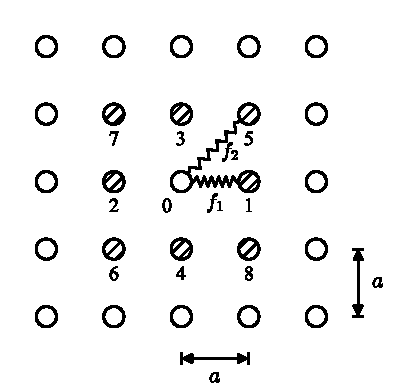
\includegraphics[width=6.5cm]{fig2-1.pdf}\\{\small 图 2.1\quad 二维正方晶格}
\end{minipage}
\end{center}

在此模型中的弹性力常数
\begin{equation}
  \Phi_{\alpha\beta}(l)=-f_l\varepsilon_{\alpha}(l)\varepsilon_{\beta}(l)
  \quad(l\neq0)
\end{equation}
其中$f_l=f_1\,(l=1,2,3,4)$，$f_l=f_2\,(l=5,6,7,8)$，$\varepsilon_{\alpha}(l)$代表沿$\boldsymbol{R}_l$方向单位矢在$\alpha$方向上的分量.对于中心原子的$\Phi_{\alpha\beta}(0)$可利用关系式(2.1.7)和(2.2.16)求得
\begin{equation}
  \Phi_{\alpha\beta}(0)=-\sum_{l\neq0}\Phi_{\alpha\beta}(l)
  =\sum_{l=1}^{8}f_l\varepsilon_l(l)\varepsilon_{\beta}(l)
\end{equation}
算出的$\Phi$矩阵为
\begin{equation}
\left.\begin{aligned}
  &\Phi(0)=2(f_1+f_2)\begin{pmatrix}1&0\\0&1\end{pmatrix}\\
  &\Phi(1)=\Phi(2)=-f_1\begin{pmatrix}1&0\\0&0\end{pmatrix},
  \quad\Phi(3)=\Phi(4)=-f_1\begin{pmatrix}0&0\\0&1\end{pmatrix}\\
  &\Phi(5)=\Phi(6)=-\frac{1}{2}f_2\begin{pmatrix}1&1\\1&1\end{pmatrix},
  \quad\Phi(7)=\Phi(8)=-\frac{1}{2}f_2\begin{pmatrix}1&-1\\-1&1\end{pmatrix}
\end{aligned}\right\}
\end{equation}
动力矩阵应由式(2.2.18)代入(2.2.3)作计算，求和限于最近邻及次近邻$(l=1,2,\cdots,8)$，即
\begin{equation}
  D(\boldsymbol{k})=\frac{2}{M}\left(\begin{array}{cc}
  \left[\begin{array}{l}f_1(1-\cos k_xa)+\\[0.3em]
  f_2(1-\cos k_xa\cos k_ya)\end{array}\right] & f_2\sin k_xa\sin k_ya\\[4ex]
  f_2\sin k_xa\sin k_ya &
  \left[\begin{array}{l}f_1(1-\cos k_ya)+\\[0.3em]
  f_2(1-\cos k_xa\cos k_ya)\end{array}\right]
  \end{array}\right)
\end{equation}
频率$\omega_{\sigma}(\boldsymbol{k})$由$D(\boldsymbol{k})$代入久期方程决定：
\begin{equation}
  \det\parallel D(\boldsymbol{k})-\omega^2I\parallel=0\,,
  \quad I=\begin{pmatrix}1&0\\0&1\end{pmatrix}
\end{equation}
根据式(2.2.19)，动力矩阵具有如下特性：
\begin{equation}
  D\Bigl(k_x+\frac{2\pi}{a},k_y+\frac{2\pi}{a}\Bigr)
  =D(k_x,k_y)=D(\boldsymbol{k})
\end{equation}
因此$\omega_{\sigma}(k_x,k_y)=\omega_{\sigma}\Bigl(k_x+\frac{2\pi}{a},k_y+\frac{2\pi}{a}\Bigr)$是倒点阵的周期函数，只需要在BZ中讨论格波.我们对于BZ中高对称点(线)上的$\omega_{\sigma}(\boldsymbol{k})$感兴趣，今分别求之：

(i)$\Sigma$线(包括$\Gamma$，M点)：令$k_x=k_y=k/\sqrt{2}$
\begin{equation}
\begin{aligned}
  \omega_1^2(\Sigma)&=\frac{2}{M}\bigg[f_1\bigg(1-\cos\frac{ka}{\sqrt{2}}\bigg)
  +f_2\bigl(1-\cos\sqrt{2}\,ka\bigr)\bigg]=\omega_{\mathrm{L}}^2(\Sigma)\\
  \omega_2^2(\Sigma)&=\frac{2}{M}f_1\bigg(1-\cos\frac{ka}{\sqrt{2}}\bigg)
  =\omega_{\mathrm{T}}^2(\Sigma)
\end{aligned}
\end{equation}
极化矢量可将以上结果代入式(2.1.13)求得
\begin{equation}
\left.\begin{aligned}
  &\boldsymbol{e}_{\Sigma1}=\Bigl(\frac{1}{\sqrt{2}},\frac{1}{\sqrt{2}}\Bigr)
  =\boldsymbol{e}_{\Sigma}^{\mathrm{L}}\\
  &\boldsymbol{e}_{\Sigma2}=\Bigl(-\frac{1}{\sqrt{2}},\frac{1}{\sqrt{2}}\Bigr)
  =\boldsymbol{e}_{\Sigma}^{\mathrm{T}}
\end{aligned}\right\}
\end{equation}
$\boldsymbol{e}_{\Sigma1}$与传播方向平行代表纵波$\boldsymbol{e}_{\Sigma}^{\mathrm{L}}$，$\boldsymbol{e}_{\Sigma2}$与传播方向相垂直为横波极化矢量$\boldsymbol{e}_{\Sigma}^{\mathrm{T}}$，如图2.2所标明.沿$\Sigma$的格波色散曲线如图2.3所示.当$4f_2>f_1$时纵波的$\omega$曲线在BZ内有极大点出现，这是与一维频谱不同之处.

\begin{center}
\begin{minipage}{6cm}
\centering
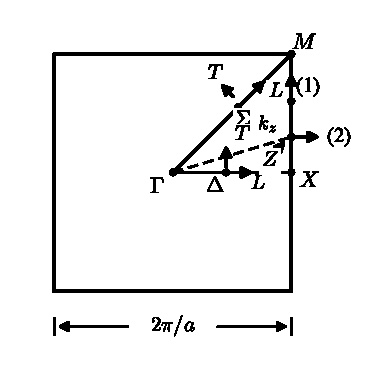
\includegraphics[width=6cm]{fig2-2.pdf}\\{\small 图 2.2\quad 二维正方晶格的极化矢量}
\end{minipage}
\end{center}

\begin{center}
\begin{minipage}{6cm}
\centering
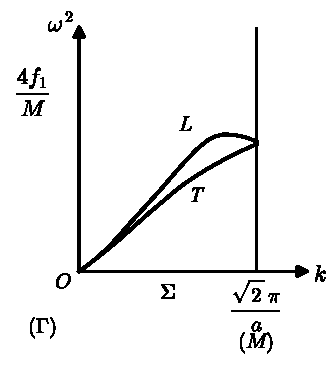
\includegraphics[width=6cm]{fig2-3.pdf}\\{\small 图 2.3}
\end{minipage}
\end{center}

(ii)$\Delta$线(包括$\Gamma$、X点)：令$k_x=k$，$k_y=0$
\begin{equation}
\begin{gathered}
  \omega_1^2(\Delta)=\frac{2}{M}(f_1+f_2)(1-\cos ka)=\omega_{\mathrm{L}}^2(\Delta)\\[1ex]
  \omega_2^2(\Delta)=\frac{2}{M}f_2(1-\cos ka)=\omega_{\mathrm{T}}^2(\Delta)
\end{gathered}
\end{equation}
\begin{equation}
  \boldsymbol{e}_{\Delta1}=(1,0)=\boldsymbol{e}_{\Delta}^{\mathrm{L}}\,,
  \quad\boldsymbol{e}_{\Delta2}=(0,1)=\boldsymbol{e}_{\Delta}^{\mathrm{T}}
\end{equation}
与$\Sigma$线相似，在$\Delta$线上纵波频率也高于横波，其色散曲线如图2.4.

(iii)Z线(包括X及M点)：令$k_x=\frac{\pi}{a}$，$k_y=k'$
\begin{equation}
\left.\begin{aligned}
  &\omega_1^2(Z)=\frac{2}{M}\bigl[2f_1+f_2(1+\cos k'a)\bigr]\\
  &\omega_2^2(Z)=\frac{2}{M}\bigl[f_1(1-\cos k'a)+f_2(1+\cos k'a)\bigr]
\end{aligned}\right\}
\end{equation}
相对应的极化矢量为
\begin{equation}
  \boldsymbol{e}_{Z1}=(0,1)\,,\quad\boldsymbol{e}_{Z2}=(1,0)
\end{equation}
它们与Z点的波矢方向($\Gamma$Z连线方向)既不平行，也不垂直.说明在Z线上的格波既非纵波，又非横波.因此，晶体中的格波只有沿某些高对称的$\boldsymbol{k}$方向传播时，才有纵横之分.这是晶体与各向同性连续介质不同之处.图2.5为沿Z方向的格波色散曲线.

从图2.3—图2.5可以看出BZ中只有在$\Gamma$与M点上纵波与横波的本征频率相同，这就是第一章§4所预言的简并情形.

\begin{center}
\begin{minipage}{6.5cm}
\centering
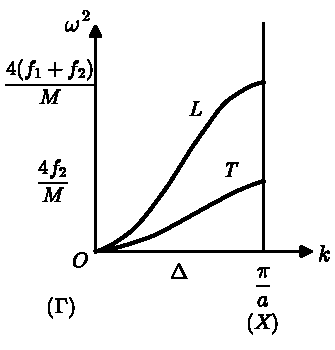
\includegraphics[width=6.5cm]{fig2-4.pdf}\\{\small 图 2.4}
\end{minipage}
\end{center}

\begin{center}
\begin{minipage}{6.5cm}
\centering
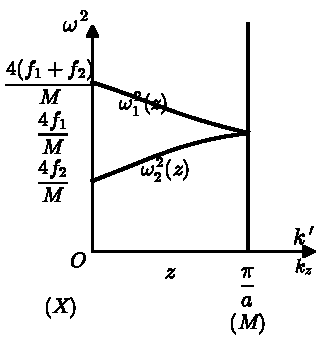
\includegraphics[width=6.5cm]{fig2-5.pdf}\\{\small 图 2.5}
\end{minipage}
\end{center}

为了熟悉复式晶格的动力矩阵$D(\boldsymbol{k})$、本征频率$\omega_{\sigma}(\boldsymbol{k})$和极化矢量$\boldsymbol{e}_{\boldsymbol{k}\sigma}(s)$的运算，我们将讨论一维复式晶格情况.

例如一维双原子链.模型如图2.6所示，两种原子$M_1$与$M_2$交替排列，近邻互作用的弹性恢复力常数分别为$f_1$和$f_2$，原胞中原子标号$s=1$，2.由于是一维，方向指标$(\alpha,\beta)$可略去.根据图中模型立刻求得$\Phi\binom{l-l'}{s,s'}$：
\begin{equation}
\left.\begin{aligned}
  &\Phi\binom{1}{1,2}=\Phi\binom{-1}{2,1}=-f_2\\
  &\Phi\binom{0}{1,2}=\Phi\binom{0}{2,1}=-f_1\\
  &\Phi\binom{0}{1,1}=-\Bigl[\Phi\binom{0}{1,2}+\Phi\binom{1}{1,2}\Bigr]
  =(f_1+f_2)=\Phi\binom{0}{2,2}
\end{aligned}\right\}
\end{equation}
其中$\Phi\binom{0}{s,s'}$利用了关系式(2.1.24)，计算准至最近邻互作用.

\begin{center}
\begin{minipage}{8cm}
\centering
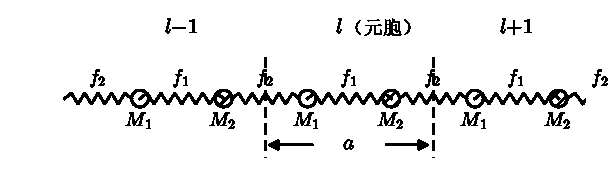
\includegraphics[width=8cm]{fig2-6.pdf}\\{\small 图 2.6\quad 一维复式晶格模型}
\end{minipage}
\end{center}

将(2.2.28)代入动力矩阵的公式(2.1.22)得到$D\binom{\boldsymbol{k}}{s,s'}\,(s,s'=1,2)$，它们组成二维矩阵
\begin{equation}
  D(\boldsymbol{k})=\left(\begin{array}{cc}
  D\binom{\boldsymbol{k}}{1,1} & D\binom{\boldsymbol{k}}{1,2}\\[1.5ex]
  D\binom{\boldsymbol{k}}{2,1} & D\binom{\boldsymbol{k}}{2,2}
  \end{array}\right)
  =\left(\begin{array}{cc}
  \dfrac{1}{M_1}(f_1+f_2) & -\dfrac{1}{\sqrt{M_1M_2}}\bigl(f_1+f_2\mathrm{e}^{-\mathrm{i}ka}\bigr)\\[3ex]
  -\dfrac{1}{\sqrt{M_1M_2}}\bigl(f_1+f_2\mathrm{e}^{\mathrm{i}ka}\bigr) & \dfrac{1}{M_2}(f_1+f_2)
  \end{array}\right)
\end{equation}
频率本征值由$\det\parallel D(\boldsymbol{k})-\omega^2I\parallel=0$决定，结果为
\begin{equation}
\begin{aligned}
  \omega_{\pm}^2(\boldsymbol{k})&=\frac{1}{2}(f_1+f_2)
  \left(\frac{1}{M_1}+\frac{1}{M_2}\right)\\
  &\quad\times\left[1\pm\sqrt{1-\frac{8f_1f_2M_1M_2}{(f_1+f_2)^2(M_1+M_2)^2}(1-\cos ka)}\,\right]
\end{aligned}
\end{equation}
有两支频谱$\omega_{\pm}^2(\boldsymbol{k})$，其中由于$\omega_-(\boldsymbol{k}=0)=0$，因此$\omega_-$就是固体物理学中的声频支格波，简称声学模，而$\omega_+$则代表光频支格波(光学模)，两支格波的色散曲线分别绘于图2.7中.

\begin{center}
\begin{minipage}{7cm}
\centering
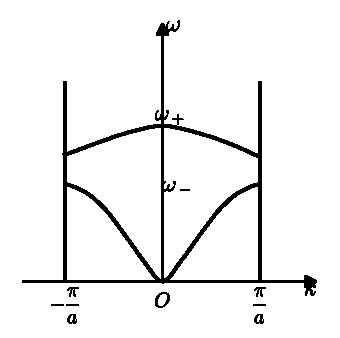
\includegraphics[width=7cm]{fig2-7.pdf}\\{\small 图 2.7}
\end{minipage}
\end{center}

$\boldsymbol{k}=0$时动力矩阵为实对称矩阵
\begin{equation}
\begin{gathered}
  D\binom{0}{1,1}=\frac{1}{M_1}(f_1+f_2)\\[1ex]
  D\binom{0}{2,2}=\frac{1}{M_2}(f_1+f_2)\\[1ex]
  D\binom{0}{1,2}=D\binom{0}{2,1}
  =-\frac{1}{\sqrt{M_1M_2}}(f_1+f_2)
\end{gathered}
\end{equation}
极化矢量$\boldsymbol{e}_{\sigma}(s)\,(\sigma=\pm\,,s=1,2)$可由式(2.1.20)决定，它们也是实量
\begin{equation}
  \boldsymbol{e}_{+}(1)=-\sqrt{\frac{M_2}{M_1}}\boldsymbol{e}_{+}(2)\,,
  \quad\boldsymbol{e}_{-}(1)=\sqrt{\frac{M_1}{M_2}}\boldsymbol{e}_{-}(2)
\end{equation}
显然，光频支振动代表元胞内$M_1$与$M_2$两原子的相对运动，其极化矢量异号，而声频支振动中两原子极化矢量同号，为同向运动，与前面的一般性讨论相符.再利用$\boldsymbol{e}_{\pm}(s)$的归一条件(2.1.27)
\begin{equation}
  e_{\pm}^2(1)+e_{\pm}^2(2)=1
\end{equation}
最后求得$\boldsymbol{k}=0$时声、光频支的极化矢量
\begin{equation}
\begin{gathered}
  \boldsymbol{e}_{+}(1)=-\frac{1}{\sqrt{\Bigl(1+\dfrac{M_1}{M_2}\Bigr)}}\,,
  \quad\boldsymbol{e}_{+}(2)=\frac{1}{\sqrt{\Bigl(1+\dfrac{M_2}{M_1}\Bigr)}}\\[3ex]
  \boldsymbol{e}_{-}(1)=\frac{1}{\sqrt{\Bigl(1+\dfrac{M_2}{M_1}\Bigr)}}\,,
  \quad\boldsymbol{e}_{-}(2)=\frac{1}{\sqrt{\Bigl(1+\dfrac{M_1}{M_2}\Bigr)}}
\end{gathered}
\end{equation}

\section{简正坐标}

在简谐近似下晶格振动已由简正模的线性叠加表示，按照式(2.1.19)其矢量形式为
\begin{equation}
  \boldsymbol{u}_l=(NM)^{-\frac{1}{2}}\sum_{\boldsymbol{k},\sigma}
  Q_{\boldsymbol{k}\sigma}\boldsymbol{e}_{\boldsymbol{k}\sigma}
  \mathrm{e}^{\mathrm{i}\boldsymbol{k}\cdot\boldsymbol{R}_l}
\end{equation}
其中$Q_{\boldsymbol{k}\sigma}$是复简正坐标，而位移$u_l^{\alpha}$为实量，这里存在一个附加条件
\begin{equation}
  \boldsymbol{e}_{\boldsymbol{k}\sigma}Q_{\boldsymbol{k}\sigma}^{*}
  =\boldsymbol{e}_{-\boldsymbol{k}\sigma}Q_{-\boldsymbol{k}\sigma}
\end{equation}
若约定极化矢量满足关系式\footnote{也可以约定$\boldsymbol{e}_{\boldsymbol{k}\sigma}=-\boldsymbol{e}_{-\boldsymbol{k}\sigma}$，则$Q_{\boldsymbol{k}\sigma}^{*}=-Q_{-\boldsymbol{k}\sigma}$，其结果相同.}
\begin{equation}
  \boldsymbol{e}_{\boldsymbol{k}\sigma}=\boldsymbol{e}_{-\boldsymbol{k}\sigma}
\end{equation}
则复简正坐标
\begin{equation}
  Q_{\boldsymbol{k}\sigma}^{*}=Q_{-\boldsymbol{k}\sigma}
\end{equation}
在简单晶体中，晶格振动的哈密顿量(2.1.8)仍为各原子位移的耦合形式，我们希望将$H$表示成各独立项相加.为此，首先用(2.3.1)将哈密顿量变换为简正坐标表示.对于动能
\begin{equation}
\begin{aligned}
  T&=\frac{1}{2}\sum_l M\dot{\boldsymbol{u}}_l\cdot\dot{\boldsymbol{u}}_l\\
  &=\frac{1}{2}\sum_{\boldsymbol{k},\boldsymbol{k}'}\sum_{\sigma,\sigma'}
  \dot{Q}_{\boldsymbol{k}'\sigma'}\dot{Q}_{\boldsymbol{k}\sigma}
  (\boldsymbol{e}_{\boldsymbol{k}'\sigma'}\cdot\boldsymbol{e}_{\boldsymbol{k}\sigma})
  \delta_{\boldsymbol{k}',-\boldsymbol{k}}\\
  &=\frac{1}{2}\sum_{\boldsymbol{k},\sigma}\sum_{\sigma'}
  \dot{Q}_{\boldsymbol{k}\sigma'}^{*}\dot{Q}_{\boldsymbol{k}\sigma}
  (\boldsymbol{e}_{\boldsymbol{k}\sigma'}\cdot\boldsymbol{e}_{\boldsymbol{k}\sigma})\\
  &=\frac{1}{2}\sum_{\boldsymbol{k},\sigma}\dot{Q}_{\boldsymbol{k}\sigma}^{*}\dot{Q}_{\boldsymbol{k}\sigma}
\end{aligned}
\end{equation}
其中利用了约定关系式(2.3.3)与(2.3.4)，本征矢量的正交关系式(2.1.16)以及当波矢限于BZ内时的关系式
\begin{equation*}
  \frac{1}{N}\sum_l\mathrm{e}^{\mathrm{i}(\boldsymbol{k}-\boldsymbol{k}')\cdot\boldsymbol{R}_l}
  =\delta_{\boldsymbol{k}'\boldsymbol{k}}
\end{equation*}
晶格振动势能在简谐近似下为
\begin{equation}
\begin{aligned}
  \Delta\Phi&=\frac{1}{2}\sum_{l,l'}\sum_{\alpha,\beta}
  u_l^{\alpha}\Phi_{\alpha\beta}(l-l')u_{l'}^{\beta}\\
  &=\frac{1}{2}\sum_{\boldsymbol{k},\boldsymbol{k}'}\sum_{\sigma,\sigma'}
  Q_{\boldsymbol{k}\sigma}^{*}Q_{\boldsymbol{k}'\sigma'}
  \frac{1}{N}\sum_l\mathrm{e}^{\mathrm{i}(\boldsymbol{k}'-\boldsymbol{k})\cdot\boldsymbol{R}_l}A
\end{aligned}
\end{equation}
其中
\begin{equation*}
\begin{aligned}
  A&=\sum_{\alpha}e_{\boldsymbol{k}\sigma}^{\alpha}\sum_{\beta}
  \Bigl\{\frac{1}{M}\sum_l\Phi_{\alpha\beta}(l-l')
  \mathrm{e}^{-\mathrm{i}\boldsymbol{k}'\cdot(\boldsymbol{R}_l-\boldsymbol{R}_{l'})}\Bigr\}
  e_{\boldsymbol{k}'\sigma'}^{\beta}\\
  &=\sum_{\alpha}e_{\boldsymbol{k}\sigma}^{\alpha}\sum_{\beta}
  D_{\alpha\beta}(\boldsymbol{k}')e_{\boldsymbol{k}'\sigma'}^{\beta}\\
  &=\Bigl(\sum_{\alpha}e_{\boldsymbol{k}\sigma}^{\alpha}e_{\boldsymbol{k}'\sigma'}^{\alpha}\Bigr)
  \omega_{\sigma'}^2(\boldsymbol{k}')
\end{aligned}
\end{equation*}
这里利用了式(2.1.12)和对角化条件式(2.1.13).将$A$代入式(2.3.6)，再利用$\boldsymbol{e}_{\boldsymbol{k}\sigma}$的正交关系式(2.1.16)，得
\begin{equation}
  \Delta\Phi=\frac{1}{2}\sum_{\boldsymbol{k},\sigma}
  \omega_{\sigma}^2(\boldsymbol{k})Q_{\boldsymbol{k}\sigma}^{*}Q_{\boldsymbol{k}\sigma}
\end{equation}
晶格振动的哈密顿量简化为
\begin{equation*}
  H=\frac{1}{2}\sum_{\boldsymbol{k},\sigma}\Bigl\{\dot{Q}_{\boldsymbol{k}\sigma}^{*}\dot{Q}_{\boldsymbol{k}\sigma}
  +\omega_{\sigma}^2(\boldsymbol{k})Q_{\boldsymbol{k}\sigma}^{*}Q_{\boldsymbol{k}\sigma}\Bigr\}
\end{equation*}
$H$在简正坐标中表示为$3N$个独立项之和，利用拉氏函数$L=T-\Delta\Phi$可求出$Q_{\boldsymbol{k}\sigma}$的共轭动量$P_{\boldsymbol{k}\sigma}$
\begin{equation}
  P_{\boldsymbol{k}\sigma}=\frac{\partial L}{\partial\dot{Q}_{\boldsymbol{k}\sigma}}
  =\dot{Q}_{\boldsymbol{k}\sigma}^{*}
\end{equation}
\begin{equation}
  H=\frac{1}{2}\sum_{\boldsymbol{k},\sigma}\Bigl\{P_{\boldsymbol{k}\sigma}^{*}P_{\boldsymbol{k}\sigma}
  +\omega_{\sigma}^2(\boldsymbol{k})Q_{\boldsymbol{k}\sigma}^{*}Q_{\boldsymbol{k}\sigma}\Bigr\}
\end{equation}
根据正则方程
\begin{equation*}
  \dot{P}_{\boldsymbol{k}\sigma}=-\frac{\partial H}{\partial Q_{\boldsymbol{k}\sigma}}
\end{equation*}
可求出简正坐标$Q_{\boldsymbol{k}\sigma}$满足方程：
\begin{equation}
  \ddot{Q}_{\boldsymbol{k}\sigma}+\omega_{\sigma}^2(\boldsymbol{k})Q_{\boldsymbol{k}\sigma}=0
\end{equation}
与简谐振子的运动方程在形式上相同，利用正交条件作式(2.3.1)的逆傅里叶变换求得简正坐标
\begin{equation}
\begin{aligned}
  Q_{\boldsymbol{k}\sigma}&=\sqrt{\frac{M}{N}}\sum_l
  (\boldsymbol{e}_{\boldsymbol{k}\sigma}\cdot\boldsymbol{u}_l)
  \mathrm{e}^{-\mathrm{i}\boldsymbol{k}\cdot\boldsymbol{R}_l}\\
  &=\frac{1}{\sqrt{NM}}\sum_{l,\alpha}Me_{\boldsymbol{k}\sigma}^{\alpha *}
  u_l^{\alpha}\mathrm{e}^{-\mathrm{i}\boldsymbol{k}\cdot\boldsymbol{R}_l}
\end{aligned}
\end{equation}
显然，$Q_{\boldsymbol{k}\sigma}$代表$N$个原子的集体振动，简正坐标是集体坐标.简正坐标$Q_{\boldsymbol{k}\sigma}$的共轭动量$P_{\boldsymbol{k}\sigma}$与第$l$个原子位移的共轭动量$\boldsymbol{p}_l=M\dot{\boldsymbol{u}}_l$之间有类似的变换关系：
\begin{equation}
  \boldsymbol{p}_l=M\dot{\boldsymbol{u}}_l=\sqrt{\frac{M}{N}}
  \sum_{\boldsymbol{k},\sigma}P_{\boldsymbol{k}\sigma}\boldsymbol{e}_{\boldsymbol{k}\sigma}
  \mathrm{e}^{-\mathrm{i}\boldsymbol{k}\cdot\boldsymbol{R}_l}
\end{equation}
其逆变换为
\begin{equation}
\begin{aligned}
  P_{\boldsymbol{k}\sigma}&=\frac{1}{\sqrt{NM}}\sum_l
  (\boldsymbol{e}_{\boldsymbol{k}\sigma}\cdot\boldsymbol{p}_l)
  \mathrm{e}^{\mathrm{i}\boldsymbol{k}\cdot\boldsymbol{R}_l}\\
  &=\frac{1}{\sqrt{NM}}\sum_{l,\alpha}e_{\boldsymbol{k}\sigma}^{\alpha *}
  p_l^{\alpha}\mathrm{e}^{\mathrm{i}\boldsymbol{k}\cdot\boldsymbol{R}_l}
\end{aligned}
\end{equation}
表明$P_{\boldsymbol{k}\sigma}$也是集体坐标.

\section{声子}

晶格振动必须用量子力学处理，其量子化条件为共轭量$p_l^{\alpha}$，$u_l^{\beta}$满足对易式
\begin{equation}
\left.\begin{aligned}
  &\bigl[p_l^{\alpha},u_{l'}^{\beta}\bigr]\equiv p_l^{\alpha}u_{l'}^{\beta}
  -u_{l'}^{\beta}p_l^{\alpha}=\frac{\hbar}{\mathrm{i}}\delta_{\alpha\beta}\delta_{ll'}\\
  &\bigl[u_l^{\alpha},u_{l'}^{\beta}\bigr]
  =\bigl[p_l^{\alpha},p_{l'}^{\beta}\bigr]=0\quad(\alpha,\beta=x,y,z)
\end{aligned}\right\}
\end{equation}
利用变换关系式(2.3.11)、(2.3.13)以及正交关系式(2.1.16)，容易由式(2.4.1)求得简正坐标$P_{\boldsymbol{k}\sigma}$、$Q_{\boldsymbol{k}\sigma}$的对易律
\begin{equation}
\left.\begin{aligned}
  [P_{\boldsymbol{k}\sigma},Q_{\boldsymbol{k}'\sigma'}]
  &=\frac{1}{N}\sum_{l,l'}\sum_{\alpha,\beta}
  \bigl(e_{\boldsymbol{k}\sigma}^{\alpha *}e_{\boldsymbol{k}'\sigma'}^{\beta}\bigr)
  \bigl[p_l^{\alpha},u_{l'}^{\beta}\bigr]
  \mathrm{e}^{\mathrm{i}(\boldsymbol{k}\cdot\boldsymbol{R}_l-\boldsymbol{k}'\cdot\boldsymbol{R}_{l'})}\\
  &=\frac{\hbar}{\mathrm{i}}\sum_{\alpha}
  \bigl(e_{\boldsymbol{k}\sigma}^{\alpha *}e_{\boldsymbol{k}'\sigma'}^{\alpha}\bigr)
  \frac{1}{N}\sum_l\mathrm{e}^{\mathrm{i}(\boldsymbol{k}-\boldsymbol{k}')\cdot\boldsymbol{R}_l}\\
  &=\frac{\hbar}{\mathrm{i}}\delta_{\sigma\sigma'}\delta_{\boldsymbol{k}\boldsymbol{k}'}\\
  [Q_{\boldsymbol{k}\sigma},Q_{\boldsymbol{k}'\sigma'}]
  &=[P_{\boldsymbol{k}\sigma},P_{\boldsymbol{k}'\sigma'}]=0
\end{aligned}\right\}
\end{equation}
应当指出在$H$的复简正坐标表式(2.3.9)中，每个单项$\frac{1}{2}\bigl\{P_{\boldsymbol{k}\sigma}^{*}P_{\boldsymbol{k}\sigma}+\omega_{\sigma}^2(\boldsymbol{k})Q_{\boldsymbol{k}\sigma}^{*}Q_{\boldsymbol{k}\sigma}\bigr\}$并不对应于量子力学中频率为$\omega_{\sigma}(\boldsymbol{k})$的简谐振子哈密顿量$\frac{1}{2}\{p^2+\omega^2q^2\}$，因为$(P,Q)$为复共轭量，而$(p,q)$为实量.根据式(2.3.4)与(2.3.8)还可以看出，式(2.3.9)实际上是
\begin{equation}
  H=\frac{1}{2}\sum_{\boldsymbol{k},\sigma}\bigl\{P_{-\boldsymbol{k}\sigma}P_{\boldsymbol{k}\sigma}
  +\omega_{\sigma}^2(\boldsymbol{k})Q_{-\boldsymbol{k}\sigma}Q_{\boldsymbol{k}\sigma}\bigr\}
\end{equation}
其中$\boldsymbol{k}$与$-\boldsymbol{k}$项仍然混杂.为消除$H$中$\boldsymbol{k}$与$-\boldsymbol{k}$的交叉项，通过正则变换定义新算符
\begin{equation}
\left.\begin{aligned}
  a_{\boldsymbol{k}\sigma}&=\sqrt{\frac{\omega_{\sigma}(\boldsymbol{k})}{2\hbar}}
  \left(Q_{\boldsymbol{k}\sigma}-\frac{P_{-\boldsymbol{k}\sigma}}{\mathrm{i}\omega_{\sigma}(\boldsymbol{k})}\right)\\[1ex]
  a_{\boldsymbol{k}\sigma}^{+}&=\sqrt{\frac{\omega_{\sigma}(\boldsymbol{k})}{2\hbar}}
  \left(Q_{-\boldsymbol{k}\sigma}+\frac{P_{\boldsymbol{k}\sigma}}{\mathrm{i}\omega_{\sigma}(\boldsymbol{k})}\right)
\end{aligned}\right\}
\end{equation}
不难验证
\begin{equation*}
\begin{aligned}
  \sum_{\boldsymbol{k},\sigma}\hbar\omega_{\sigma}(\boldsymbol{k})a_{\boldsymbol{k}\sigma}^{+}a_{\boldsymbol{k}\sigma}
  &=\frac{1}{2}\sum_{\boldsymbol{k},\sigma}\bigl\{P_{-\boldsymbol{k}\sigma}P_{\boldsymbol{k}\sigma}
  +\omega_{\sigma}^2(\boldsymbol{k})Q_{-\boldsymbol{k}\sigma}Q_{\boldsymbol{k}\sigma}\bigr\}\\
  &\quad-\mathrm{i}\frac{1}{2}\sum_{\boldsymbol{k},\sigma}\omega_{\sigma}(\boldsymbol{k})
  \bigl[P_{\boldsymbol{k}\sigma},Q_{\boldsymbol{k}\sigma}\bigr]\\
  &=H-\frac{1}{2}\sum_{\boldsymbol{k},\sigma}\hbar\omega_{\sigma}(\boldsymbol{k})
\end{aligned}
\end{equation*}
推导时只用了对易式(2.4.2)与频率的普遍关系式$\omega_{\sigma}(\boldsymbol{k})=\omega_{\sigma}(-\boldsymbol{k})$.用新算符$a_{\boldsymbol{k}\sigma}$表示的$H$为下列不含$\boldsymbol{k}$与$-\boldsymbol{k}$交叉项的对角形式
\begin{equation}
  H=\sum_{\boldsymbol{k},\sigma}\left(a_{\boldsymbol{k}\sigma}^{+}a_{\boldsymbol{k}\sigma}
  +\frac{1}{2}\right)\hbar\omega_{\sigma}(\boldsymbol{k})
  =\sum_{\boldsymbol{k},\sigma}H_{\boldsymbol{k}\sigma}
\end{equation}
对易关系为
\begin{equation}
\begin{aligned}
  &\bigl[a_{\boldsymbol{k}\sigma},a_{\boldsymbol{k}'\sigma'}^{+}\bigr]
  =\delta_{\sigma\sigma'}\delta_{\boldsymbol{k}\boldsymbol{k}'}\\
  &\bigl[a_{\boldsymbol{k}\sigma},a_{\boldsymbol{k}'\sigma'}\bigr]
  =\bigl[a_{\boldsymbol{k}\sigma}^{+},a_{\boldsymbol{k}'\sigma'}^{+}\bigr]=0
\end{aligned}
\end{equation}
用$a_{\boldsymbol{k}\sigma}$及$a_{\boldsymbol{k}\sigma}^{+}$表示的位移得
\begin{equation}
  \boldsymbol{u}_l=\sum_{\boldsymbol{k},\sigma}
  \left(\frac{\hbar}{2NM\omega_{\sigma}(\boldsymbol{k})}\right)^{\frac{1}{2}}
  \boldsymbol{e}_{\boldsymbol{k}\sigma}
  \bigl\{a_{\boldsymbol{k}\sigma}\mathrm{e}^{\mathrm{i}\boldsymbol{k}\cdot\boldsymbol{R}_l}
  +a_{\boldsymbol{k}\sigma}^{+}\mathrm{e}^{-\mathrm{i}\boldsymbol{k}\cdot\boldsymbol{R}_l}\bigr\}
\end{equation}
其时间依赖关系可利用海森伯运动方程
\begin{equation*}
\begin{aligned}
  \dot{a}_{\boldsymbol{k}\sigma}&=\frac{\mathrm{i}}{\hbar}[H,a_{\boldsymbol{k}\sigma}]
  =-\mathrm{i}\omega_{\sigma}(\boldsymbol{k})a_{\boldsymbol{k}\sigma}\\
  a_{\boldsymbol{k}\sigma}&=a_{\boldsymbol{k}}(0)\mathrm{e}^{-\mathrm{i}\omega_{\sigma}(\boldsymbol{k})t}
\end{aligned}
\end{equation*}
代入式(2.4.7)，得
\begin{equation*}
\begin{aligned}
  \boldsymbol{u}_l(t)&=\sum_{\boldsymbol{k},\sigma}
  \left(\frac{\hbar}{2NM\omega_{\sigma}(\boldsymbol{k})}\right)^{\frac{1}{2}}
  \boldsymbol{e}_{\boldsymbol{k}\sigma}
  \bigl\{a_{\boldsymbol{k}\sigma}(0)
  \mathrm{e}^{\mathrm{i}[\boldsymbol{k}\cdot\boldsymbol{R}_l-\omega_{\sigma}(\boldsymbol{k})t]}\\
  &\quad+a_{\boldsymbol{k}\sigma}^{+}(0)
  \mathrm{e}^{-\mathrm{i}[\boldsymbol{k}\cdot\boldsymbol{R}_l-\omega_{\sigma}(\boldsymbol{k})t]}\bigr\}\\
  &=\sum_{\boldsymbol{k},\sigma}
  \left(\frac{\hbar}{2NM\omega_{\sigma}(\boldsymbol{k})}\right)^{\frac{1}{2}}
  \boldsymbol{e}_{\boldsymbol{k}\sigma}\bigl\{a_{\boldsymbol{k}\sigma}(0)
  \mathrm{e}^{\mathrm{i}[\boldsymbol{k}\cdot\boldsymbol{R}_l-\omega_{\sigma}(\boldsymbol{k})t]}
  +\mathrm{h.c.}\bigr\}
\end{aligned}
\end{equation*}
其中h.c.代表厄米共轭项.这是位移的行波展式，其中每一求和项代表频率$\omega_{\sigma}(\boldsymbol{k})$、偏振$\boldsymbol{e}_{\boldsymbol{k}\sigma}$、沿$\boldsymbol{k}$方向传播的格波，它所对应的哈密顿量是$H_{\boldsymbol{k}\sigma}$.不难证明，定态薛定谔方程
\begin{equation}
  H_{\boldsymbol{k}\sigma}\psi_{\boldsymbol{k}\sigma}
  =\varepsilon_{\boldsymbol{k}\sigma}\psi_{\boldsymbol{k}\sigma}\,,
  \quad H_{\boldsymbol{k}\sigma}\equiv
  \left(a_{\boldsymbol{k}\sigma}^{+}a_{\boldsymbol{k}\sigma}+\frac{1}{2}\right)
  \hbar\omega_{\sigma}(\boldsymbol{k})
\end{equation}
的解$\varepsilon_{\boldsymbol{k}\sigma}$与频率为$\omega_{\sigma}(\boldsymbol{k})$的简谐振子能量形式相同.式(2.4.8)可等效地写为
\begin{equation}
  \hbar\omega_{\sigma}(\boldsymbol{k})a_{\boldsymbol{k}\sigma}^{+}a_{\boldsymbol{k}\sigma}
  \psi_{\boldsymbol{k}\sigma}
  =\Bigl[\varepsilon_{\boldsymbol{k}\sigma}
  -\frac{1}{2}\hbar\omega_{\sigma}(\boldsymbol{k})\Bigr]\psi_{\boldsymbol{k}\sigma}
  \equiv\varepsilon'_{\boldsymbol{k}\sigma}\psi_{\boldsymbol{k}\sigma}
\end{equation}
为书写简便起见，暂略去脚标$(\boldsymbol{k},\sigma)$，将上式写成
\begin{equation}
  \hbar\omega a^{+}a\psi=\varepsilon'\psi
\end{equation}
下面分别讨论算符方程式(2.4.10)的基态和激发态：

\subsection*{(i) 基态}

设基态为$\psi_0$，有能量$\varepsilon'_0$，它应当是具有最低能量的状态，采用狄拉克(Dirac)符号，用$\lvert0\rangle$表示$\psi_0$，则有等式
\begin{equation}
  \hbar\omega a^{+}a\lvert0\rangle=\varepsilon'_0\lvert0\rangle
\end{equation}
将算符$a$作用于此等式两边，并利用对易式(2.4.6)
\begin{equation*}
  \hbar\omega aa^{+}a\lvert0\rangle
  =\hbar\omega\bigl(a^{+}a+1\bigr)a\lvert0\rangle
  =\varepsilon'_0a\lvert0\rangle
\end{equation*}
得到另一个状态$a\lvert0\rangle$满足
\begin{equation*}
  \hbar\omega a^{+}a\bigl(a\lvert0\rangle\bigr)
  =(\varepsilon'_0-\hbar\omega)\bigl(a\lvert0\rangle\bigr)
\end{equation*}
当$\omega>0$时它比$\lvert0\rangle$态具有更低能量，显然与原假设矛盾.所以，基态必需满足条件
\begin{equation}
  a\lvert0\rangle=0
\end{equation}
上式即二次量子化表象中的基态定义.由此可知$a^{+}a\lvert0\rangle=0$，代入式(2.4.11)得$\varepsilon'_0=0$，于是基态能
\begin{equation}
  \varepsilon_0=\frac{1}{2}\hbar\omega
\end{equation}
它相当于振子的零点能.

\subsection*{(ii) 激发态}

用算符$a^{+}$作用于基态，再利用对易关系，可求出等式
\begin{equation}
  \hbar\omega a^{+}a\bigl(a^{+}\lvert0\rangle\bigr)
  =\hbar\omega\bigl(a^{+}\lvert0\rangle\bigr)
\end{equation}
$a^{+}\lvert0\rangle$代表激发一个格波量子$\hbar\omega$的状态，称为第一激发态.若用$(a^{+})^n$作用，则得到
\begin{equation*}
  \hbar\omega a^{+}a\bigl\{(a^{+})^n\lvert0\rangle\bigr\}
  =n\hbar\omega\bigl\{(a^{+})^n\lvert0\rangle\bigr\}
\end{equation*}
因此$(a^{+})^n\lvert0\rangle$代表激发$n$个格波量子的状态，叫做第$n$激发态，并采用记号$\lvert n\rangle$表示
\begin{equation}
  \lvert n\rangle=c_n(a^{+})^n\lvert0\rangle
\end{equation}
其中$c_n$由归一条件决定.这样就得到式(2.4.10)的解为
\begin{equation*}
\begin{gathered}
  \hbar\omega a^{+}a\lvert n\rangle=\varepsilon'_n\lvert n\rangle\\[1ex]
  \varepsilon'_n=n\hbar\omega\quad(n=1,2,3,\cdots)
\end{gathered}
\end{equation*}
由此可见，格波能量总是以量子$\hbar\omega$一份份地激发，这个量子称为声子.激发了$n$个声子的$\omega$格波能量为
\begin{equation}
  \varepsilon_n=\varepsilon'_n+\frac{1}{2}\hbar\omega
  =\left(n+\frac{1}{2}\right)\hbar\omega
\end{equation}
与谐振子的能量一致.

\subsection*{(iii) 递推关系}

根据式(2.4.15)，可令
\begin{equation*}
  \lvert n\rangle=\lambda_na^{+}\lvert n-1\rangle
\end{equation*}
则求得
\begin{equation*}
\begin{aligned}
  \langle n\vert n\rangle&=|\lambda_n|^2\langle n-1\vert
  \bigl(aa^{+}\bigr)\vert n-1\rangle\\
  &=|\lambda_n|^2n\langle n-1\vert n-1\rangle
\end{aligned}
\end{equation*}
由于$\lvert n\rangle$与$\lvert n-1\rangle$都应当满足归一条件
\begin{equation*}
  \langle n\vert n\rangle=1\,,\quad\langle n-1\vert n-1\rangle=1
\end{equation*}
因此
\begin{equation*}
  \lambda_n=n^{-\frac{1}{2}}
\end{equation*}
并求出递推公式
\begin{equation}
  \lvert n\rangle=n^{-\frac{1}{2}}a^{+}\lvert n-1\rangle
\end{equation}
从递推公式(2.4.17)即可导出重要关系式
\begin{equation}
\left.\begin{aligned}
  &a^{+}\lvert n\rangle=\sqrt{n+1}\,\lvert n+1\rangle\\
  &a\lvert n\rangle=\sqrt{n}\,\lvert n-1\rangle
\end{aligned}\right\}
\end{equation}
上式说明$a^{+}$代表声子的产生算符，它使格波从$n$个声子态变为$(n+1)$个声子状态，而$a$算符使格波从$n$变为$(n-1)$个声子的状态，称为声子的消灭算符.算符
\begin{equation}
  \hat{n}\equiv a^{+}a
\end{equation}
有特性
\begin{equation}
  \hat{n}\lvert n\rangle=a^{+}a\lvert n\rangle=n\lvert n\rangle
  \quad(n=0,1,2,\cdots)
\end{equation}
其本征值为$n$，代表声子数，因此$\hat{n}$称为声子数算符.

以上讨论的优点是，无需具体给出$\lvert0\rangle$的表示式，就可以求得格波激发态的全部信息.$\lvert n\rangle$是用声子数算符本征值标记的状态，它就是希尔伯特空间中的态向量.

利用递推公式还可定出
\begin{equation}
\begin{gathered}
  c_n=\lambda_1\cdot\lambda_2\cdots\lambda_n=(n!)^{-\frac{1}{2}}\\[1ex]
  \lvert n\rangle=\frac{1}{\sqrt{n!}}(a^{+})^n\lvert0\rangle
\end{gathered}
\end{equation}
现在恢复脚标$(\boldsymbol{k},\sigma)$，讨论总哈密顿量$H$的本征能量.由于$k\sigma$格波的哈密顿量为$H_{\boldsymbol{k}\sigma}=\left(a_{\boldsymbol{k}\sigma}^{+}a_{\boldsymbol{k}\sigma}+\frac{1}{2}\right)\allowbreak\hbar\omega_{\sigma}(\boldsymbol{k})$，当状态用声子数标记为$\lvert n_{\boldsymbol{k}\sigma}\rangle$时，有能量$\varepsilon_{\boldsymbol{k}\sigma}=\left(n_{\boldsymbol{k}\sigma}+\frac{1}{2}\right)\hbar\omega_{\sigma}(\boldsymbol{k})$.因此
\begin{equation}
  H=\sum_{\boldsymbol{k},\sigma}H_{\boldsymbol{k}\sigma}
  =\sum_{\boldsymbol{k},\sigma}\left(a_{\boldsymbol{k}\sigma}^{+}a_{\boldsymbol{k}\sigma}
  +\frac{1}{2}\right)\hbar\omega_{\sigma}(\boldsymbol{k})
\end{equation}
代表$3N$种不同$(\boldsymbol{k},\sigma)$的无互作用声子系统，而总能量为
\begin{equation}
  E=\sum_{\boldsymbol{k},\sigma}\hbar\omega_{\sigma}(\boldsymbol{k})
  \left(n_{\boldsymbol{k}\sigma}+\frac{1}{2}\right)
\end{equation}
说明晶格振动的激发状态，在物理上可以用$3N$个独立格波的声子数组态$\lvert\{n_{\boldsymbol{k}\sigma}\}\rangle$表示.由于声子算符满足玻色对易式(2.4.6)，它是玻色粒子.式(2.4.22)与(2.4.23)代表理想玻色气体的$H$和$E$.这样，$N$个原子(离子)的耦合振荡问题在简谐近似下约化为独立玻色子系统.温度为$T$时，$(k\sigma)$格波所激发的平均声子数按玻色统计为
\begin{equation}
  \bar{n}_{\boldsymbol{k}\sigma}
  =\frac{1}{\exp\bigl[\hbar\omega_{\sigma}(\boldsymbol{k})/k_{\mathrm{B}}T\bigr]-1}
\end{equation}
当$T=0\,$K时，所有$(\boldsymbol{k},\sigma)$态上的声子数均为零，称为声子的真空，这时只有晶格振动的零点能.引入声子概念便于处理固体中相互作用问题，例如在声子-声子、电子-声子、光子-声子等互作用过程中，把声子当作有能量$\hbar\omega_{\sigma}(\boldsymbol{k})$和动量$\hbar\boldsymbol{k}$的玻色粒子来处理，将是十分方便的.但是，应当明白声子并不是一个真正的粒子，声子可以产生和消灭，有相互作用时声子数不守恒，声子动量的守恒律也不同于一般粒子，并且声子不能脱离固体存在.声子只是格波激发的量子，在多体理论中称为集体振荡的元激发或准粒子.

\section{长波方法(一)——声学模}

在多数问题中，长波长的声子起重要作用.为此，有必要单独讨论晶格动力学理论的长波极限$(\boldsymbol{k}\to0)$情况.由于声频支代表同一元胞中诸原子(基元)的质心运动，因此复式晶格中声学模也可以当简单晶格处理，只需认为$M$是元胞中原子的总质量.

对于长波长的晶格振动，其振幅在元胞间缓慢变化，晶体结构的原子性对问题影响不大，可以过渡到连续介质模型.

引入一个在空间缓变的位移场$\boldsymbol{u}(\boldsymbol{r})$代表$\boldsymbol{r}$点附近小体元的位移.当$\boldsymbol{r}=\boldsymbol{R}_l$(简记为$r=l$)时，$\boldsymbol{u}$就是$l$元胞中质心的位移
\begin{equation}
  u_l^{\alpha}=u^{\alpha}(\boldsymbol{r})\big|_{r=l}
\end{equation}
$\boldsymbol{u}$当然也是时间$t$的函数，而无需标明.考虑到振幅$u_l^{\alpha}$在元胞间缓慢变化，可将位移场作泰勒展开得到近似式
\begin{equation}
  u_{l'}^{\alpha}=u_l^{\alpha}
  +\sum_{\mu}\bigl(\boldsymbol{R}_{l'}-\boldsymbol{R}_l\bigr)_{\mu}
  \frac{\partial u^{\alpha}(\boldsymbol{r})}{\partial r_{\mu}}\bigg|_{r=l}
\end{equation}
式(2.5.1)与(2.5.2)是过渡到连续介质模型的基本关系式，此外还需定义密度
\begin{equation}
  \rho=\frac{M}{\Omega}
\end{equation}
和利用求和与积分的变换
\begin{equation}
  \Omega\sum_l\left(\cdots\right)=\int\mathrm{d}\tau\left(\cdots\right)
\end{equation}
可把晶格振动的动能按照式(2.5.1)与(2.5.4)改写为
\begin{equation*}
\begin{aligned}
  T&=\frac{1}{2}\sum_l M|\dot{\boldsymbol{u}}_l|^2\\
  &=\Omega\sum_l\frac{1}{2}\rho|\dot{\boldsymbol{u}}(\boldsymbol{r}=l)|^2\\
  &=\int\mathrm{d}\tau\Bigl\{\frac{1}{2}\rho|\dot{\boldsymbol{u}}(\boldsymbol{r})|^2\Bigr\}\\
  &=\int\mathrm{d}\tau\,\mathscr{T}(\boldsymbol{r})
\end{aligned}
\end{equation*}
其中
\begin{equation}
  \mathscr{T}(\boldsymbol{r})=\frac{1}{2}\rho|\dot{\boldsymbol{u}}(\boldsymbol{r})|^2
  =\frac{1}{2}\rho\sum_{\alpha}\dot{u}^{\alpha}\dot{u}^{\alpha}
\end{equation}
代表动能密度.晶格振动的位能比较复杂.首先利用式(2.1.7)和点阵具有反演对称性
\begin{equation}
  \Phi_{\alpha\beta}(l-l')=\Phi_{\alpha\beta}(l'-l)
\end{equation}
将$\Phi$的表示式(2.1.3)改写为对称的形式
\begin{equation}
  \Delta\Phi=-\frac{1}{4}\sum_{\alpha,\beta}\sum_{l,l'}
  \bigl(u_{l'}^{\alpha}-u_l^{\alpha}\bigr)\Phi_{\alpha\beta}(l-l')
  \bigl(u_{l'}^{\beta}-u_l^{\beta}\bigr)
\end{equation}
再将式(2.5.2)代入
\begin{equation}
\begin{aligned}
  \Delta\Phi&=\frac{1}{2}\Omega\sum_l\sum_{\alpha,\beta}\sum_{\mu,\nu}
  C_{\alpha\beta;\mu\nu}
  \frac{\partial u^{\alpha}(\boldsymbol{r})}{\partial r_{\mu}}\bigg|_{r=l}\cdot
  \frac{\partial u^{\beta}(\boldsymbol{r})}{\partial r_{\nu}}\bigg|_{r=l}\\
  &=\int\mathrm{d}\tau\sum_{\alpha,\beta}\sum_{\mu,\nu}
  \frac{1}{2}C_{\alpha\beta;\mu\nu}
  \frac{\partial u^{\alpha}}{\partial r_{\mu}}\frac{\partial u^{\beta}}{\partial r_{\nu}}
\end{aligned}
\end{equation}
其中定义系数
\begin{equation}
  C_{\alpha\beta;\mu\nu}\equiv-\frac{1}{2\Omega}\sum_{l'}
  \Phi_{\alpha\beta}(l-l')
  \bigl(\boldsymbol{R}_{l'}-\boldsymbol{R}_l\bigr)_{\mu}
  \bigl(\boldsymbol{R}_{l'}-\boldsymbol{R}_l\bigr)_{\nu}
\end{equation}
由式(2.5.8)和$\Delta\Phi=\int\mathrm{d}\tau\,\phi(\boldsymbol{r})$，求得势能密度
\begin{equation}
  \phi(\boldsymbol{r})=\sum_{\alpha,\beta}\sum_{\mu,\nu}
  \frac{1}{2}C_{\alpha\beta;\mu\nu}
  \frac{\partial u^{\alpha}}{\partial r_{\mu}}\frac{\partial u^{\beta}}{\partial r_{\nu}}
\end{equation}
它是应变$\frac{\partial u^{\alpha}}{\partial r_{\mu}}$的二次函数.$\phi(\boldsymbol{r})$又称为形变能密度，$C_{\alpha\beta;\mu\nu}$称为弹性系数.

具体求解弹性问题时，首先应考虑对称性，并找出弹性系数之间的对称关系，从而简化$\phi(\boldsymbol{r})$的表示式.最简单而又最常用的模型是把晶体当作弹性各向同性体.这时弹性能与取向无关，式(2.5.10)绕任意轴旋转应当不变.由于位移场$\boldsymbol{u}(\boldsymbol{r})$只可能有$\nabla\cdot\boldsymbol{u}$、$\nabla\boldsymbol{u}$及$\nabla\times\boldsymbol{u}$三种一阶导数，因此能保持上述旋转不变性的二次函数只可能是它们的标量二次型：$(\nabla\cdot\boldsymbol{u})^2$、$|\nabla\boldsymbol{u}|^2$和$|\nabla\times\boldsymbol{u}|^2$，其中$\nabla\times\boldsymbol{u}$代表晶体旋转，而不是应变，这一项不会在弹性能中出现.因此，弹性各向同性体的形变能密度应具有下列简单形式：
\begin{equation}
\begin{aligned}
  \phi(\boldsymbol{r})&=\frac{1}{2}A(\nabla\cdot\boldsymbol{u})^2
  +\frac{1}{2}B|\nabla\boldsymbol{u}|^2\\
  &=\frac{1}{2}A\sum_{\alpha,\beta}
  \frac{\partial u^{\alpha}}{\partial r_{\alpha}}\frac{\partial u^{\beta}}{\partial r_{\beta}}
  +\frac{1}{2}B\sum_{\alpha,\mu}
  \frac{\partial u^{\alpha}}{\partial r_{\mu}}\frac{\partial u^{\alpha}}{\partial r_{\mu}}
\end{aligned}
\end{equation}
与式(2.5.10)相比较，求得$A$，$B$与弹性系数的关系为
\begin{equation}
  C_{\alpha\beta,\mu\nu}=A\delta_{\alpha\mu}\delta_{\beta\nu}
  +B\delta_{\alpha\beta}\delta_{\mu\nu}
\end{equation}
长波近似的动力矩阵由式(2.1.12)对小$k$展开求得
\begin{equation}
\begin{aligned}
  D_{\alpha\beta}&=\frac{1}{M}\sum_l\Phi_{\alpha\beta}(l)
  \Bigl\{1-\mathrm{i}\boldsymbol{k}\cdot\boldsymbol{R}_l
  -\frac{1}{2}(\boldsymbol{k}\cdot\boldsymbol{R}_l)^2+\cdots\Bigr\}\\
  &=\frac{1}{2M}\sum_{\mu,\nu}\sum_l\Phi_{\alpha\beta}(\boldsymbol{l})
  l_{\mu}l_{\nu}k_{\mu}k_{\nu}\\
  &=\frac{1}{\rho}\sum_{\mu,\nu}C_{\alpha\beta;\mu\nu}k_{\mu}k_{\nu}
\end{aligned}
\end{equation}
其中$l_{\mu}$代表$(\boldsymbol{R}_l)_{\mu}$，在推导时也同样利用了式(2.1.7)和(2.5.6).将式(2.5.13)代入本征方程式(2.1.13)，求得长波情况下的本征方程为
\begin{equation}
  \rho\omega^2e_{\boldsymbol{k}}^{\alpha}
  =\sum_{\beta}\sum_{\mu,\nu}C_{\alpha\beta;\mu\nu}
  k_{\mu}k_{\nu}e_{\boldsymbol{k}}^{\beta}
\end{equation}
$\omega$是$\boldsymbol{k}$的线性函数，并且当$\boldsymbol{k}=0$时$\omega=0$，具有声频支解的特征，对于弹性各向同性体利用式(2.5.12)可进一步简化本征方程
\begin{equation}
  \rho\omega^2e_{\boldsymbol{k}}^{\alpha}
  =A\sum_{\beta}k_{\alpha}k_{\beta}e_{\boldsymbol{k}}^{\beta}
  +Bk^2e_{\boldsymbol{k}}^{\alpha}
\end{equation}
式(2.5.15)的矢量表示式为
\begin{equation}
  \rho\omega^2\boldsymbol{e}_{\boldsymbol{k}}
  =A(\boldsymbol{k}\cdot\boldsymbol{e}_{\boldsymbol{k}})\boldsymbol{k}
  +Bk^2\boldsymbol{e}_{\boldsymbol{k}}
\end{equation}
它有一个纵波$(\boldsymbol{k}\parallel\boldsymbol{e}_{\boldsymbol{k}})$解和两个横波$(\boldsymbol{k}\perp\boldsymbol{e}_{\boldsymbol{k}})$的解
\begin{equation}
  \omega_{\mathrm{L}}=c_{\mathrm{L}}k\,,\quad
  c_{\mathrm{L}}=\sqrt{(A+B)/\rho}
\end{equation}
\begin{equation}
  \omega_{\mathrm{T}}=c_{\mathrm{T}}k\,,\quad
  c_{\mathrm{T}}=\sqrt{B/\rho}
\end{equation}
横波声速$c_{\mathrm{T}}$小于纵波声速$c_{\mathrm{L}}$.

由于求本征方程时实际上是假定了$\exp[\mathrm{i}(\boldsymbol{k}\cdot\boldsymbol{r}-\omega t)]$形式的解(参见§1)，因此作下列对应：
\begin{equation*}
  -\mathrm{i}\omega\to\frac{\partial}{\partial t}\,;\quad
  \mathrm{i}k_{\mu}\to\frac{\partial}{\partial r_{\mu}}\,;\quad
  e_{\boldsymbol{k}}^{\alpha}\to u^{\alpha}
\end{equation*}
这可使我们立刻求得弹性波方程
\begin{equation}
  \rho\ddot{u}^{\alpha}=\sum_{\beta}\sum_{\mu,\nu}C_{\alpha\beta;\mu\nu}
  \frac{\partial^2u^{\beta}}{\partial r_{\mu}\partial r_{\nu}}
\end{equation}
当然，严格的作法应从$\mathscr{L}=\mathscr{T}-\phi$的拉格朗日方程导出.当各向同性时有
\begin{equation}
  \rho\ddot{u}^{\alpha}=A\sum_{\beta}
  \frac{\partial^2u^{\beta}}{\partial r_{\alpha}\partial r_{\beta}}
  +B\sum_{\beta}\frac{\partial^2u^{\alpha}}{\partial r_{\beta}^2}
  \quad(\alpha,\beta=x,y,z)
\end{equation}
略经变化可求得矢量表示式
\begin{equation}
  \ddot{\boldsymbol{u}}=c_{\mathrm{T}}^2\nabla^2\boldsymbol{u}
  +\bigl(c_{\mathrm{L}}^2-c_{\mathrm{T}}^2\bigr)\nabla(\nabla\cdot\boldsymbol{u})
\end{equation}
这就是人们熟知的弹性波方程.

各向同性连续介质的哈密顿量为
\begin{equation}
  H=\int_V\mathrm{d}\tau\biggl\{\frac{1}{2\rho}\sum_{\alpha}p^{\alpha}p^{\alpha}
  +\frac{1}{2}A\sum_{\alpha,\beta}
  \frac{\partial u^{\alpha}}{\partial r_{\alpha}}\frac{\partial u^{\beta}}{\partial r_{\beta}}
  +\frac{1}{2}B\sum_{\alpha,\beta}
  \frac{\partial u^{\alpha}}{\partial r_{\beta}}\frac{\partial u^{\alpha}}{\partial r_{\beta}}\biggr\}
\end{equation}
其中
\begin{equation}
  p^{\alpha}=\frac{\partial\mathscr{L}}{\partial\dot{u}^{\alpha}}
  =\frac{\partial(\mathscr{T}-\phi)}{\partial\dot{u}^{\alpha}}
  =\rho\dot{u}^{\alpha}
\end{equation}
是$u^{\alpha}$的共轭动量，类似于本章§3中方法引入简正坐标
\begin{equation}
\left.\begin{aligned}
  \boldsymbol{u}(\boldsymbol{r})&=\frac{1}{\sqrt{\rho V}}
  \sum_{\boldsymbol{k},\sigma}\boldsymbol{e}_{\boldsymbol{k}\sigma}Q_{\boldsymbol{k}\sigma}
  \mathrm{e}^{\mathrm{i}\boldsymbol{k}\cdot\boldsymbol{r}}\\
  \boldsymbol{p}(\boldsymbol{r})&=\sqrt{\frac{\rho}{V}}
  \sum_{\boldsymbol{k},\sigma}\boldsymbol{e}_{\boldsymbol{k}\sigma}P_{\boldsymbol{k}\sigma}
  \mathrm{e}^{-\mathrm{i}\boldsymbol{k}\cdot\boldsymbol{r}}
\end{aligned}\right\}
\end{equation}
其中$P_{\boldsymbol{k}\sigma}$为$Q_{\boldsymbol{k}\sigma}$的共轭动量，它等于$\dot{Q}_{\boldsymbol{k}\sigma}^{*}$.此外，约定关系式(2.3.3)和(2.3.4)保持不变.将式(2.5.24)代入式(2.5.22)，利用极化矢量的正交条件和关系式
\begin{equation}
  \frac{1}{V}\int_V\mathrm{d}\tau\,
  \mathrm{e}^{\mathrm{i}(\boldsymbol{k}+\boldsymbol{k}')\cdot\boldsymbol{r}}
  =\delta_{\boldsymbol{k}',-\boldsymbol{k}}
\end{equation}
求得
\begin{equation*}
  H=\frac{1}{2}\sum_{\boldsymbol{k},\sigma}
  \Bigl\{P_{-\boldsymbol{k}\sigma}P_{\boldsymbol{k}\sigma}
  +\frac{1}{\rho}\bigl[A(\boldsymbol{k}\cdot\boldsymbol{e}_{\boldsymbol{k}\sigma})
  (\boldsymbol{k}\cdot\boldsymbol{e}_{\boldsymbol{k}\sigma'})
  Q_{-\boldsymbol{k}\sigma}Q_{\boldsymbol{k}\sigma}
  +Bk^2Q_{-\boldsymbol{k}\sigma}Q_{\boldsymbol{k}\sigma}\bigr]\Bigr\}
\end{equation*}
再借助于本征方程式(2.5.16)
\begin{equation}
\begin{aligned}
  A(\boldsymbol{k}\cdot\boldsymbol{e}_{\boldsymbol{k}\sigma})
  (\boldsymbol{k}\cdot\boldsymbol{e}_{\boldsymbol{k}\sigma'})
  &=\bigl[\rho\omega_{\sigma}^2(\boldsymbol{k})-Bk^2\bigr]
  (\boldsymbol{e}_{\boldsymbol{k}\sigma}\cdot\boldsymbol{e}_{\boldsymbol{k}\sigma'})\\
  &=\bigl[\rho\omega_{\sigma}^2(\boldsymbol{k})-Bk^2\bigr]\delta_{\sigma\sigma'}
\end{aligned}
\end{equation}
最后得到哈密顿量的简正坐标表示
\begin{equation}
  H=\frac{1}{2}\sum_{\boldsymbol{k},\sigma}
  \bigl\{P_{-\boldsymbol{k}\sigma}P_{\boldsymbol{k}\sigma}
  +\omega_{\sigma}^2(\boldsymbol{k})Q_{-\boldsymbol{k}\sigma}Q_{\boldsymbol{k}\sigma}\bigr\}
\end{equation}
再作变换，引入声子的产生及消灭算符
\begin{equation}
  H=\sum_{\boldsymbol{k},\sigma}\hbar\omega_{\sigma}(\boldsymbol{k})
  \left(a_{\boldsymbol{k}\sigma}^{+}a_{\boldsymbol{k}\sigma}+\frac{1}{2}\right)
\end{equation}
其中$\omega_{\sigma}(\boldsymbol{k})$有一个纵波和两个横波解，如式(2.5.17)和(2.5.18)所示.根据变换式(2.4.4)，将简正坐标
\begin{equation}
  Q_{\boldsymbol{k}\sigma}=\sqrt{\frac{\hbar}{2\omega_{\sigma}(\boldsymbol{k})}}
  \bigl(a_{\boldsymbol{k}\sigma}+a_{-\boldsymbol{k}\sigma}^{+}\bigr)
\end{equation}
代入式(2.5.24)，求得位移场的二次量子化表示式
\begin{equation}
  \boldsymbol{u}(\boldsymbol{r})=\sum_{\boldsymbol{k},\sigma}
  \boldsymbol{e}_{\boldsymbol{k}\sigma}
  \sqrt{\frac{\hbar}{2\rho\omega_{\sigma}(\boldsymbol{k})V}}
  \bigl(a_{\boldsymbol{k}\sigma}\mathrm{e}^{\mathrm{i}\boldsymbol{k}\cdot\boldsymbol{r}}
  +a_{\boldsymbol{k}\sigma}^{+}\mathrm{e}^{-\mathrm{i}\boldsymbol{k}\cdot\boldsymbol{r}}\bigr)
\end{equation}
位移场的散度与体积变化有关\footnote{由于单位体积经形变，体积膨胀为
$1+\delta V=\left(1+\frac{\partial u^x}{\partial x}\right)
\left(1+\frac{\partial u^y}{\partial y}\right)
\left(1+\frac{\partial u^z}{\partial z}\right)
\approx1+\sum_{\alpha}\frac{\partial u^{\alpha}}{\partial r_{\alpha}}$，
因此体积的相对变化为
$\Delta=\frac{\delta V}{V}=\frac{\partial u^x}{\partial x}
+\frac{\partial u^y}{\partial y}
+\frac{\partial u^z}{\partial z}=\nabla\cdot\boldsymbol{u}$.}，由上式容易得到体积的相对变化为
\begin{equation}
\begin{aligned}
  \Delta(\boldsymbol{r})&=\nabla\cdot\boldsymbol{u}\\
  &=\mathrm{i}\sum_{\boldsymbol{k},\sigma}
  \sqrt{\frac{\hbar}{2\rho\omega_{\sigma}(\boldsymbol{k})V}}
  (\boldsymbol{e}_{\boldsymbol{k}\sigma}\cdot\boldsymbol{k})
  \bigl(a_{\boldsymbol{k}\sigma}\mathrm{e}^{\mathrm{i}\boldsymbol{k}\cdot\boldsymbol{r}}
  -a_{\boldsymbol{k}\sigma}^{+}\mathrm{e}^{-\mathrm{i}\boldsymbol{k}\cdot\boldsymbol{r}}\bigr)\\
  &=\mathrm{i}\sum_{\boldsymbol{k}}
  \sqrt{\frac{\hbar}{2\rho V\omega_{\mathrm{L}}(\boldsymbol{k})}}\,k
  \bigl(a_{\boldsymbol{k}\mathrm{L}}\mathrm{e}^{\mathrm{i}\boldsymbol{k}\cdot\boldsymbol{r}}
  -a_{\boldsymbol{k}\mathrm{L}}^{+}\mathrm{e}^{-\mathrm{i}\boldsymbol{k}\cdot\boldsymbol{r}}\bigr)
\end{aligned}
\end{equation}
这个表示式说明只有纵波导致体积变化.因此，LA声子对电子的互作用将比TA声子更重要.

\section{长波方法(二)——光学模}

在离子晶体中长波光学模代表元胞内正、负离子的反方向运动，它伴随着极化并与电磁波有强烈的相互作用，从而对离子晶体的电学与光学特性有重要影响.本节介绍黄昆的长波方法\textsuperscript{[1]}，它将告诉我们如何由离子晶体的宏观特性确定长光学模频率.

为简单起见，设每个元胞中只含两个电荷量相等、符号相反的离子，仍限于各向同性连续模型.由于在长波限各元胞中正、负离子的相对位移$(\boldsymbol{u}_{+}-\boldsymbol{u}_{-})$几乎一样，因此可以用一个矢量$\boldsymbol{W}$描述光频支振动
\begin{equation}
  \boldsymbol{W}\equiv\rho^{\frac{1}{2}}(\boldsymbol{u}_{+}-\boldsymbol{u}_{-})
\end{equation}
这里$\rho$代表折合质量的密度
\begin{equation}
  \rho=\frac{M}{\Omega}\,,\quad
  M=\frac{M_{+}M_{-}}{M_{+}+M_{-}}
\end{equation}
$M_{\pm}$为正、负离子的质量，$M$是折合质量.矢量$\boldsymbol{W}$可称为折合位移.光频支振动的动能密度
\begin{equation}
  \mathscr{T}=\frac{1}{2}\dot{\boldsymbol{W}}\cdot\dot{\boldsymbol{W}}
\end{equation}
位能密度由两部分组成，即
\begin{equation*}
  \phi=\phi_{\text{弹性}}+\phi_{\text{极化}}
\end{equation*}
弹性能可设为
\begin{equation}
  \phi_{\text{弹性}}=\frac{1}{2}\gamma_{11}\boldsymbol{W}\cdot\boldsymbol{W}
\end{equation}
极化部分由公式
\begin{equation}
  \phi_{\text{极化}}=-\int_0^{E}\boldsymbol{P}\cdot\mathrm{d}\boldsymbol{E}
\end{equation}
决定，其中$\boldsymbol{P}$代表晶体的极化强度，$\boldsymbol{E}$为宏观电场.显然正、负离子的相对位移导致极化并产生内场，这个场又反过来作用于离子影响它们的运动，并且还使离子上电子相对于核位移产生电子极化.因此极化强度应表示为
\begin{equation}
  \boldsymbol{P}=\gamma_{12}\boldsymbol{W}+\gamma_{22}\boldsymbol{E}
\end{equation}
上式右边第一项为离子位移极化，第二项与离子上电子极化有关.把式(2.6.6)代入式(2.6.5)，求得极化所产生的位能
\begin{equation}
  \phi_{\text{极化}}
  =-\Bigl(\gamma_{12}\boldsymbol{W}\cdot\boldsymbol{E}
  +\frac{1}{2}\gamma_{22}\boldsymbol{E}\cdot\boldsymbol{E}\Bigr)
\end{equation}
而总位能密度为
\begin{equation}
  \phi=\Bigl(\frac{1}{2}\gamma_{11}\boldsymbol{W}\cdot\boldsymbol{W}
  -\gamma_{12}\boldsymbol{W}\cdot\boldsymbol{E}
  -\frac{1}{2}\gamma_{22}\boldsymbol{E}\cdot\boldsymbol{E}\Bigr)
\end{equation}
其中$\gamma_{ij}\,(\gamma_{ij}=\gamma_{ji})$为待定系数.上式可理解为，在各向同性时总位能密度是两个场量$\boldsymbol{W}$和$\boldsymbol{E}$的标量二次型.拉氏量密度$\mathscr{L}$由$\mathscr{T}-\phi$组成
\begin{equation}
  \mathscr{L}=\frac{1}{2}\dot{\boldsymbol{W}}\cdot\dot{\boldsymbol{W}}
  -\Bigl(\frac{1}{2}\gamma_{11}\boldsymbol{W}\cdot\boldsymbol{W}
  -\gamma_{12}\boldsymbol{W}\cdot\boldsymbol{E}
  -\frac{1}{2}\gamma_{22}\boldsymbol{E}\cdot\boldsymbol{E}\Bigr)
\end{equation}
根据上式可确定位移$\boldsymbol{W}$的共轭动量为
\begin{equation*}
  \frac{\partial\mathscr{L}}{\partial\dot{\boldsymbol{W}}}=\dot{\boldsymbol{W}}
\end{equation*}
因此哈密顿密度为
\begin{equation}
  \mathscr{H}=\frac{1}{2}\dot{\boldsymbol{W}}\cdot\dot{\boldsymbol{W}}
  +\Bigl(\frac{1}{2}\gamma_{11}\boldsymbol{W}\cdot\boldsymbol{W}
  -\gamma_{12}\boldsymbol{W}\cdot\boldsymbol{E}
  -\frac{1}{2}\gamma_{22}\boldsymbol{E}\cdot\boldsymbol{E}\Bigr)
\end{equation}
对上式利用正则方程，可导出光学模的运动方程
\begin{equation}
  \ddot{\boldsymbol{W}}=-\gamma_{11}\boldsymbol{W}+\gamma_{12}\boldsymbol{E}
\end{equation}
其中右边第一项代表弹性恢复力，是短程作用，第二项是极化所产生宏观内场对离子运动的作用力，它概括了长程作用.长波方法的优点就在于用宏观内场代替对离子间的长程库仑力求和.式(2.6.6)与式(2.6.11)是长波方法的两个基本方程，称为黄昆方程.利用这套方程可求出离子晶体中光学模的横波(TO)与纵波(LO)频率，并且诸系数$\gamma_{ij}$均可由常用的宏观测量值决定(如高、低频介电常数$\varepsilon_{\infty}$、$\varepsilon_0$等).

\subsection*{1. 介电函数}

3个待定系数$\gamma_{11}$，$\gamma_{12}$，$\gamma_{22}$与介电函数有关.考虑$\boldsymbol{E}$、$\boldsymbol{P}$、$\boldsymbol{W}$的平面波解，当$\boldsymbol{k}=0$时写为
\begin{equation}
  \boldsymbol{E}=\boldsymbol{E}_0\mathrm{e}^{-\mathrm{i}\omega t}\,,\quad
  \boldsymbol{P}=\boldsymbol{P}_0\mathrm{e}^{-\mathrm{i}\omega t}\,,\quad
  \boldsymbol{W}=\boldsymbol{W}_0\mathrm{e}^{-\mathrm{i}\omega t}
\end{equation}
代入式(2.6.6)与式(2.6.11)求得
\begin{equation}
\left.\begin{aligned}
  &-\omega^2\boldsymbol{W}=-\gamma_{11}\boldsymbol{W}+\gamma_{12}\boldsymbol{E}\\
  &\boldsymbol{P}=\gamma_{12}\boldsymbol{W}+\gamma_{22}\boldsymbol{E}
\end{aligned}\right\}
\end{equation}
消去$\boldsymbol{W}$后得到
\begin{equation}
  \boldsymbol{P}=\biggl\{\gamma_{22}+\frac{\gamma_{12}^2}{\gamma_{11}-\omega^2}\biggr\}\boldsymbol{E}
\end{equation}
根据
\begin{equation*}
  \boldsymbol{D}=\boldsymbol{E}+4\pi\boldsymbol{P}=\varepsilon\boldsymbol{E}
\end{equation*}
可求出$\varepsilon$与$\omega$有关的表示式
\begin{equation}
  \varepsilon(\omega)=1+4\pi\biggl\{\gamma_{22}
  +\frac{\gamma_{12}^2}{\gamma_{11}-\omega^2}\biggr\}
\end{equation}
$\varepsilon(\omega)$称为介电函数.介电函数在$\omega^2=\omega_0^2=\gamma_{11}$时有极点，因此$\gamma_{11}$由$\varepsilon(\omega)$的极点$\omega_0$决定，$\omega_0$在红外区域.$\omega\ll\omega_0$时的$\varepsilon$值即为熟知的静态介电常数$\varepsilon_0$，根据式(2.6.15)静态介电常数
\begin{equation}
  \varepsilon_0=1+4\pi\Biggl(\gamma_{22}+\frac{\gamma_{12}^2}{\gamma_{11}}\Biggr)
\end{equation}
当$\omega\gg\omega_0$时，$\varepsilon=\varepsilon_{\infty}$，$\varepsilon_{\infty}$称为高频介电常数，可得到关系式
\begin{equation}
  \varepsilon_{\infty}=1+4\pi\gamma_{22}
\end{equation}
于是求得诸系数$\gamma_{ij}$
\begin{equation}
\left.\begin{aligned}
  &\gamma_{11}=\omega_0^2\\
  &\gamma_{12}=\left(\frac{\varepsilon_0-\varepsilon_{\infty}}{4\pi}\right)^{\frac{1}{2}}\omega_0\\
  &\gamma_{22}=\frac{\varepsilon_{\infty}-1}{4\pi}
\end{aligned}\right\}
\end{equation}
由此得到介电函数的表示式为
\begin{equation}
  \varepsilon(\omega)=\varepsilon_{\infty}
  +\frac{\varepsilon_0-\varepsilon_{\infty}}{\omega_0^2-\omega^2}\,\omega_0^2
\end{equation}

\subsection*{2. 横波及纵波振动方程}

在各向同性介质中，光学模可划分为纵波部分与横波部分.对于矢量$\boldsymbol{W}$、$\boldsymbol{P}$、$\boldsymbol{E}$也可作相应的划分
\begin{equation}
\left.\begin{aligned}
  &\boldsymbol{W}=\boldsymbol{W}_{\mathrm{T}}+\boldsymbol{W}_{\mathrm{L}}\,,\quad
  \nabla\cdot\boldsymbol{W}_{\mathrm{T}}=0\,,\quad\nabla\times\boldsymbol{W}_{\mathrm{L}}=0\\
  &\boldsymbol{E}=\boldsymbol{E}_{\mathrm{T}}+\boldsymbol{E}_{\mathrm{L}}\,,\quad
  \nabla\cdot\boldsymbol{E}_{\mathrm{T}}=0\,,\quad\nabla\times\boldsymbol{E}_{\mathrm{L}}=0\\
  &\boldsymbol{P}=\boldsymbol{P}_{\mathrm{T}}+\boldsymbol{P}_{\mathrm{L}}\,,\quad
  \nabla\cdot\boldsymbol{P}_{\mathrm{T}}=0\,,\quad\nabla\times\boldsymbol{P}_{\mathrm{L}}=0
\end{aligned}\right\}
\end{equation}
因此式(2.6.11)写为
\begin{equation}
  \ddot{\boldsymbol{W}}_{\mathrm{T(L)}}+\gamma_{11}\boldsymbol{W}_{\mathrm{T(L)}}
  =\gamma_{12}\boldsymbol{E}_{\mathrm{T(L)}}
\end{equation}
当不存在外电磁场时，$\nabla\times\boldsymbol{E}_{\mathrm{T}}
=-\frac{1}{c}\frac{\partial\boldsymbol{B}}{\partial t}=0$，又由于$\nabla\cdot\boldsymbol{E}_{\mathrm{T}}=0$，因此$\boldsymbol{E}_{\mathrm{T}}=0$，横振动方程变为
\begin{equation}
  \ddot{\boldsymbol{W}}_{\mathrm{T}}+\omega_{\mathrm{T}}^2\boldsymbol{W}_{\mathrm{T}}=0\,,
  \quad\omega_{\mathrm{T}}^2=\gamma_{11}=\omega_0^2
\end{equation}
注意，横波频率与介电函数的极点频率$\omega_0$相等.

对于纵振动，场$\boldsymbol{E}_{\mathrm{L}}\neq0$，应确定$\boldsymbol{E}_{\mathrm{L}}$与$\boldsymbol{W}_{\mathrm{L}}$的关系.考虑到离子晶格中平均电荷密度为零，故
$\nabla\cdot\boldsymbol{D}=\nabla\cdot(\boldsymbol{E}_{\mathrm{L}}+4\pi\boldsymbol{P}_{\mathrm{L}})=0$，
又因为$\nabla\times(\boldsymbol{E}_{\mathrm{L}}+4\pi\boldsymbol{P}_{\mathrm{L}})=0$，所以
\begin{equation}
  \boldsymbol{E}_{\mathrm{L}}+4\pi\boldsymbol{P}_{\mathrm{L}}=0
\end{equation}
再利用宏观方程式(2.6.6)，得到关系式
\begin{equation}
  \boldsymbol{E}_{\mathrm{L}}
  =-\frac{4\pi\gamma_{12}}{1+4\pi\gamma_{22}}\boldsymbol{W}_{\mathrm{L}}
\end{equation}
代入式(2.6.21)，求出纵波本征方程
\begin{equation}
  \ddot{\boldsymbol{W}}_{\mathrm{L}}+\omega_{\mathrm{L}}^2\boldsymbol{W}_{\mathrm{L}}=0
\end{equation}
其中纵振动频率为
\begin{equation}
  \omega_{\mathrm{L}}^2=\gamma_{11}+\frac{4\pi\gamma_{12}^2}{1+4\pi\gamma_{22}}
\end{equation}
再把式(2.6.22)和(2.6.18)代入上式，可求出纵波与横波频率关系为
\begin{equation}
  \omega_{\mathrm{L}}^2=\frac{\varepsilon_0}{\varepsilon_{\infty}}\,\omega_{\mathrm{T}}^2
\end{equation}
这就是著名的LST[利顿(Lyddane)—萨克斯(Sachs)—特勒(Teller)]关系.

利用LST关系改写式(2.6.15)，可将介电函数明确表示为
\begin{equation}
  \varepsilon(\omega)=\varepsilon_{\infty}
  \frac{\omega_{\mathrm{L}}^2-\omega^2}{\omega_{\mathrm{T}}^2-\omega^2}
\end{equation}
由上式可以看出，$\omega_{\mathrm{L}}$为介电函数的零点频率，$\omega_{\mathrm{T}}$为$\varepsilon(\omega)$的极点.由于$\varepsilon_0>\varepsilon_{\infty}$，从LST关系得知，$\omega_{\mathrm{L}}>\omega_{\mathrm{T}}$.因此，当$\omega_{\mathrm{T}}<\omega<\omega_{\mathrm{L}}$时，$\varepsilon(\omega)<0$.如果电磁波频率在$\varepsilon(\omega)$的极点与零点之间，则它只能在晶体边界上被反射，而不能在介质中传播.$\omega_{\mathrm{L}}$称为反射区上界，$\omega_{\mathrm{T}}$则为其下界，这些量很容易由光学方法测定.

\section{极化激元}

现在研究光学模与电磁波的相互作用.由于光子是横向电磁场的量子，光照射离子晶体时将激发横向电磁场，从而对离子晶体中光频支横波振动产生影响.特别是当光子频率$\omega=kc$与横波光学模声子(TO声子)的频率$\omega_{\mathrm{T}}$(约$10^{13}\,\mathrm{s}^{-1}$)相近时，两者的耦合很强，其结果将使光子与TO声子的色散曲线都发生很大的改变，形成光子—横光学模声子的耦合模式，其量子称为极化激元(polaritons)，是离子晶体中的元激发.由于$\omega=\omega_{\mathrm{T}}$时对应的光子波数
$k=\frac{\omega}{c}=\frac{\omega_{\mathrm{T}}}{c}$(约$10^3\,\mathrm{cm}^{-1}$)与布里渊区的尺寸(约$10^8\,\mathrm{cm}^{-1}$)相比为小量，属于长波范围，因此极化激元是长波长横向光频支振动与电磁场的耦合模量子.

为了求出耦合模，必须考虑黄昆方程与电磁场麦克斯韦方程的联立解
\begin{equation}
\left.\begin{aligned}
  &\nabla\times\boldsymbol{E}_{\mathrm{T}}=-\frac{1}{c}\dot{\boldsymbol{H}}\\
  &\nabla\times\boldsymbol{H}=\frac{1}{c}
  (\dot{\boldsymbol{E}}_{\mathrm{T}}+4\pi\dot{\boldsymbol{P}}_{\mathrm{T}})\\
  &\boldsymbol{P}_{\mathrm{T}}=\gamma_{12}\boldsymbol{W}_{\mathrm{T}}
  +\gamma_{22}\boldsymbol{E}_{\mathrm{T}}\\
  &\ddot{\boldsymbol{W}}_{\mathrm{T}}+\omega_{\mathrm{T}}^2\boldsymbol{W}_{\mathrm{T}}
  -\gamma_{12}\boldsymbol{E}_{\mathrm{T}}=0
\end{aligned}\right\}
\end{equation}
其中假定：(i)介质是非磁性的，因此$\nabla\cdot\boldsymbol{H}=0$.(ii)不存在空间电流，$j=0$.(iii)无自由电荷，$\nabla\cdot(\boldsymbol{E}+4\pi\boldsymbol{P})
=\nabla\cdot(\boldsymbol{E}_{\mathrm{L}}+4\pi\boldsymbol{P}_{\mathrm{L}})=0$，因此式(2.6.23)仍成立.由于式(2.7.1)仅涉及横向场量，为简单起见下面将略去场量的脚标T.

考虑平面波型解，并设波矢$\boldsymbol{k}$沿$z$方向，$\boldsymbol{E}$、$\boldsymbol{P}$、$\boldsymbol{W}$在$x$方向振动，而$\boldsymbol{H}$沿$y$方向
\begin{equation}
  \frac{E_x}{E_x(0)}=\frac{P_x}{P_x(0)}=\frac{W_x}{W_x(0)}
  =\frac{H_y}{H_y(0)}=\exp[\mathrm{i}(kz-\omega t)]
\end{equation}
代入式(2.7.1)，求得线性方程组
\begin{equation}
\left.\begin{aligned}
  &kE_x-\frac{\omega}{c}H_y=0\\
  &\frac{\omega}{c}E_x-kH_y+\frac{4\pi\omega}{c}P_x=0\\
  &-\gamma_{22}E_x+P_x-\gamma_{12}W_x=0\\
  &-\gamma_{12}E_x+(\omega_{\mathrm{T}}^2-\omega^2)W_x=0
\end{aligned}\right\}
\end{equation}
耦合模式的本征频率由式(2.7.3)的系数行列式等于零决定.利用式(2.6.18)和式(2.6.27)可将频率方程写为
\begin{equation}
  \varepsilon_{\infty}\omega^4
  -\bigl(\varepsilon_{\infty}\omega_{\mathrm{L}}^2+k^2c^2\bigr)\omega^2
  +k^2c^2\omega_{\mathrm{T}}^2=0
\end{equation}
由上式解得极化激元的色散曲线为
\begin{equation}
  \omega^2=\frac{1}{2}\Biggl\{\omega_{\mathrm{L}}^2+\frac{k^2c^2}{\varepsilon_{\infty}}
  \pm\biggl[\omega_{\mathrm{L}}^4+\frac{k^4c^4}{\varepsilon_{\infty}^2}
  +\frac{2k^2c^2}{\varepsilon_{\infty}}\bigl(\omega_{\mathrm{L}}^2-2\omega_{\mathrm{T}}^2\bigr)
  \biggr]^{1/2}\Biggr\}
\end{equation}
极化激元的解分$\omega_{\pm}(k)$两支，当$k\to0$时
\begin{equation}
  \omega_{+}^2\approx\omega_{\mathrm{L}}^2\,,\quad
  \omega_{-}^2\approx\frac{k^2c^2}{\varepsilon_0}
\end{equation}
当$k\gg\frac{\omega_{\mathrm{L}}}{c}\sqrt{\varepsilon_{\infty}}$时
\begin{equation}
  \omega_{+}^2\approx\frac{k^2c^2}{\varepsilon_{\infty}}\,,\quad
  \omega_{-}^2\approx\omega_{\mathrm{T}}^2
\end{equation}
$\omega_{\pm}(k)$有二重根，说明存在两种横波，它们的偏振方向不同，但频率相同.

图2.8绘出了两支极化激元的色散曲线，它们分布在
\begin{equation*}
  0<\omega_-(k)<\omega_{\mathrm{T}}\,,\quad
  \omega_{\mathrm{L}}<\omega_+(k)<\infty
\end{equation*}
两段频区内.在$\omega_{\mathrm{T}}<\omega<\omega_{\mathrm{L}}$频率范围内不存在耦合模的传播解，代表禁区，$\omega_+$支与$\omega_-$支被禁区隔开.更细致的分析图2.8还可以看出$\omega_+$与$\omega_-$有下列特征：

(i)对于大$k$值，$\omega_-$解即是原来的TO声子频率，而$\omega_+$解则代表光速为$\frac{c}{\sqrt{\varepsilon_{\infty}}}$的光子频率.这时可以说$\omega_-$支类似声子，$\omega_+$支类似光子.

(ii)对于小$k$值，$\omega_-$支变成代表介质中光速为$\frac{c}{\sqrt{\varepsilon_0}}$的光子，而$\omega_+$支则与$\omega_{\mathrm{L}}$频率的TO声子类似.这时与情况(i)相反，两支解变为$\omega_-$类光及$\omega_+$类声.

(iii)对于$k$值的中间区域，$\omega_+$与$\omega_-$既不类光也不类声.

因此，从$\omega_+$和$\omega_-$的整个曲线看，不能认定$\omega_+$及$\omega_-$中哪一支类光，哪一支类声，反映出$\omega_{\pm}$具有声子与光子耦合模的特征.

\begin{center}
\begin{minipage}{7cm}
\centering
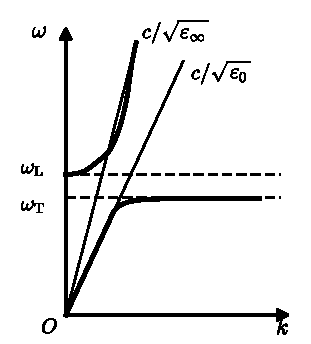
\includegraphics[width=7cm]{fig2-8.pdf}\\{\small 图 2.8\quad 极化激元的色散曲线}
\end{minipage}
\end{center}

\begin{center}
\begin{minipage}{6cm}
\centering
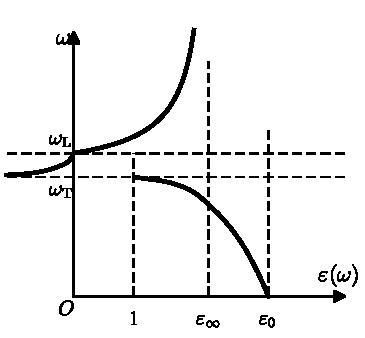
\includegraphics[width=6cm]{fig2-9.pdf}\\{\small 图 2.9\quad 极化激元的介电函数}
\end{minipage}
\end{center}

\begin{center}
\begin{minipage}{6cm}
\centering
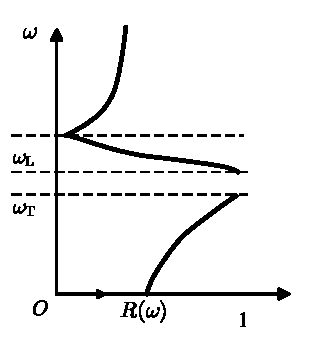
\includegraphics[width=6cm]{fig2-10.pdf}\\{\small 图 2.10\quad 反射比曲线}
\end{minipage}
\end{center}

利用式(2.7.4)与式(2.6.28)，可以导出极化激元的介电函数$\varepsilon(\omega)$与频率关系为
\begin{equation}
  \frac{k^2c^2}{\omega^2}=\varepsilon_{\infty}
  \frac{\omega_{\mathrm{L}}^2-\omega^2}{\omega_{\mathrm{T}}^2-\omega^2}
  =\varepsilon(\omega)
\end{equation}
图2.9是根据上式所作的$\varepsilon(\omega)$曲线.显然，在$\omega_{\mathrm{T}}<\omega<\omega_{\mathrm{L}}$频率范围内，介电函数取负值，它正好与耦合模的禁带相重合.当$\varepsilon(\omega)<0$时，由式(2.7.8)求得的$k$是纯虚数，代表指数衰减解，说明入射光不能在离子晶体中传播，与此同时实验上将观测到强烈的反射现象.例如，设晶体占据$z>0$半空间，对于沿正$z$方向垂直入射的电磁波，入射波的波数为$\frac{\omega}{c}$，而且入射的电场和磁场为
\begin{equation}
  E_x^{\mathrm{i}}=H_y^{\mathrm{i}}=A\mathrm{e}^{\mathrm{i}\omega\left(\frac{z}{c}-t\right)}
  \quad(z<0)
\end{equation}
由于在晶体界面上的反射波沿负$z$方向，其电场与磁场关系应设为
\begin{equation}
  E_x^{\mathrm{r}}=-H_y^{\mathrm{r}}\quad(z<0)
\end{equation}
为了决定$E_x^{\mathrm{r}}$及$H_y^{\mathrm{r}}$，我们还应当利用晶体中的极化激元解和$E_x$、$H_y$在真空与晶体界面两侧的连续条件.由式(2.7.2)和式(2.7.8)得到晶体中极化激元的电场为
\begin{equation}
  E_x=E_x(0)\mathrm{e}^{\mathrm{i}(kz-\omega t)}\quad(z>0)
\end{equation}
\begin{equation}
  k=\frac{\omega}{c}\sqrt{\varepsilon(\omega)}
\end{equation}
晶体中的$H_y$可从式(2.7.1)的第一个公式求得
\begin{equation}
  H_y=\sqrt{\varepsilon(\omega)}\,E_x\quad(z>0)
\end{equation}
再利用$z=0$界面两侧$E_x$与$H_y$的连续条件
\begin{equation}
\begin{gathered}
  E_x^{\mathrm{i}}+E_x^{\mathrm{r}}=E_x(0)\\[1ex]
  E_x^{\mathrm{i}}-E_x^{\mathrm{r}}=\sqrt{\varepsilon(\omega)}\,E_x(0)
\end{gathered}
\end{equation}
消去$E_x(0)$，求得入射波与反射波在界面上满足关系
\begin{equation}
  \frac{E_x^{\mathrm{i}}-E_x^{\mathrm{r}}}{E_x^{\mathrm{i}}+E_x^{\mathrm{r}}}
  =\sqrt{\varepsilon(\omega)}
\end{equation}
实验上测量的反射比定义为
\begin{equation}
  R(\omega)\equiv\biggl|\frac{E_x^{\mathrm{r}}}{E_x^{\mathrm{i}}}\biggr|^2
\end{equation}
它代表反射和入射电磁波在$z=0$处的强度比.由此立刻导出垂直入射时的反射比公式
\begin{equation}
  R(\omega)\equiv\biggl|
  \frac{\sqrt{\varepsilon(\omega)}-1}{\sqrt{\varepsilon(\omega)}+1}
  \biggr|^2
\end{equation}
从上式可知，当$\varepsilon(\omega)<0$时，$R(\omega)=1$，这时垂直入射的电磁波将在离子晶体表面被完全反射(图2.10)，与此同时在晶体中恰好没有极化激元的传播模式.以上讨论说明极化激元对于解释晶体中的光学现象起重要作用.

上述讨论表明：必须用TO声子与光子间耦合模(极化激元)的色散曲线才能全面解释电磁波在离子晶体中的传播特性.20世纪70年代以来，极化激元概念已推广到电磁波与固体中(包括表面、界面和超晶格)一切电性与磁性集体激发的线性耦合系统.人们将光子与TO声子、激子和磁振子等的耦合模量子都称作极化激元，并已为拉曼(Raman)光谱实验所证实.

\section{态密度}

当讨论晶体热力学性质时，往往涉及到对于各种独立格波的$(\boldsymbol{k},\sigma)$求和.由于波矢$\boldsymbol{k}$呈准连续分布，每一频带内的格波频率$\omega_{\sigma}(\boldsymbol{k})$也将是准连续分布的，因此在具体计算热力学量时，可以把$(\boldsymbol{k},\sigma)$的求和变换为对频率的积分，并同时引进态密度.平均每个元胞(或格点)的态密度$g(\omega)$定义为单位频率间隔内的格波模式数被总元胞数$N$除.对于三维复式晶体，当元胞内含有$s$个原子时，态密度的积分应等于平均每个元胞内的振动自由度$3s$.
\begin{equation}
  \int_0^{\infty}g(\omega)\mathrm{d}\omega=3s
\end{equation}
$g(\omega)$的具体表示式从晶格自由能引入.由于$(\boldsymbol{k},\sigma)$格波在简谐近似下的振动能量为
$\hbar\omega_{\sigma}(\boldsymbol{k})\left(n_{\boldsymbol{k}\sigma}+\frac{1}{2}\right)$，
其中$n_{\boldsymbol{k}\sigma}$为$(\boldsymbol{k},\sigma)$格波上激发的声子数.因此，声子数组态为$\{n_{\boldsymbol{k}\sigma}\}$时，系统的总振动能量为
\begin{equation*}
  E_{\{n_{\boldsymbol{k}\sigma}\}}
  =\sum_{\boldsymbol{k},\sigma}\hbar\omega_{\sigma}(\boldsymbol{k})
  \left(n_{\boldsymbol{k}\sigma}+\frac{1}{2}\right)
\end{equation*}
晶格振动的配分函数为
\begin{equation}
  Z=\sum_{\{n_{\boldsymbol{k}\sigma}\}}
  \exp(-\beta E_{\{n_{\boldsymbol{k}\sigma}\}})
  =\prod_{\boldsymbol{k},\sigma}
  \frac{\mathrm{e}^{-\frac{1}{2}\beta\hbar\omega_{\sigma}(\boldsymbol{k})}}
  {1-\mathrm{e}^{-\beta\hbar\omega_{\sigma}(\boldsymbol{k})}}
\end{equation}
其中$\beta=(1/k_{\mathrm{B}}T)$.按照热力学公式，不难从式(2.8.2)算得自由能
\begin{equation}
  F=-k_{\mathrm{B}}T\ln Z
  =k_{\mathrm{B}}T\sum_{\boldsymbol{k},\sigma}
  \ln\biggl[2\sinh\frac{\hbar\omega_{\sigma}(\boldsymbol{k})}{2k_{\mathrm{B}}T}\biggr]
\end{equation}
利用狄拉克$\delta$函数的特性
\begin{equation}
  f\bigl[\omega_{\sigma}(\boldsymbol{k})\bigr]
  \delta\bigl[\omega-\omega_{\sigma}(\boldsymbol{k})\bigr]
  =f(\omega)\delta\bigl[\omega-\omega_{\sigma}(\boldsymbol{k})\bigr]
\end{equation}
以及
\begin{equation}
  \int_0^{\infty}\delta\bigl[\omega-\omega_{\sigma}(\boldsymbol{k})\bigr]\mathrm{d}\omega=1
\end{equation}
可以将自由能公式(2.8.3)中的$\boldsymbol{k}$求和变换为对$\omega$的下列积分
\begin{equation}
\begin{aligned}
  F&=Nk_{\mathrm{B}}T\int_0^{\infty}
  \ln\Bigl[2\sinh\frac{\hbar\omega}{2k_{\mathrm{B}}T}\Bigr]
  \biggl\{\frac{1}{N}\sum_{\boldsymbol{k},\sigma}
  \delta\bigl[\omega-\omega_{\sigma}(\boldsymbol{k})\bigr]\biggr\}\mathrm{d}\omega\\
  &=Nk_{\mathrm{B}}T\int_0^{\infty}
  \ln\Bigl[2\sinh\frac{\hbar\omega}{2k_{\mathrm{B}}T}\Bigr]g(\omega)\mathrm{d}\omega
\end{aligned}
\end{equation}
其中
\begin{equation}
  g(\omega)\equiv\frac{1}{N}\sum_{\boldsymbol{k},\sigma}
  \delta\bigl[\omega-\omega_{\sigma}(\boldsymbol{k})\bigr]
\end{equation}
利用式(2.8.5)，容易证明所导出的态密度公式(2.8.7)满足关系式(2.8.1)，因为
\begin{equation*}
  \int_0^{\infty}g(\omega)\mathrm{d}\omega
  =\frac{1}{N}\sum_{\boldsymbol{k},\sigma}\int_0^{\infty}
  \delta\bigl[\omega-\omega_{\sigma}(\boldsymbol{k})\bigr]\mathrm{d}\omega
  =\frac{1}{N}\Bigl(\sum_{\boldsymbol{k},\sigma}1\Bigr)
  =\Bigl(\sum_{\sigma}1\Bigr)=3s
\end{equation*}
因此，式(2.8.7)给出晶格系统的正确态密度公式.

态密度$g(\omega)$是计算晶格热力学特性的重要物理量.利用式(2.8.6)可以求出晶格振动的内能$U$，热容$C_V$和熵$S$为
\begin{equation}
  U=F-T\Bigl(\frac{\partial F}{\partial T}\Bigr)_V
  =N\int_0^{\infty}\frac{1}{2}\hbar\omega
  \coth\Bigl(\frac{\hbar\omega}{2k_{\mathrm{B}}T}\Bigr)g(\omega)\mathrm{d}\omega
\end{equation}
\begin{equation}
  C_V=\Bigl(\frac{\partial U}{\partial T}\Bigr)_V
  =Nk_{\mathrm{B}}\int_0^{\infty}
  \left(\frac{\hbar\omega}{2k_{\mathrm{B}}T}\right)^2
  \mathrm{csch}^2\biggl(\frac{\hbar\omega}{2k_{\mathrm{B}}T}\biggr)
  g(\omega)\mathrm{d}\omega
\end{equation}
\begin{equation}
  S=-\Bigl(\frac{\partial F}{\partial T}\Bigr)_V
  =Nk_{\mathrm{B}}\int_0^{\infty}
  \biggl\{\frac{\hbar\omega}{2k_{\mathrm{B}}T}
  \coth\biggl(\frac{\hbar\omega}{2k_{\mathrm{B}}T}\biggr)
  -\ln\biggl[2\sinh\biggl(\frac{\hbar\omega}{2k_{\mathrm{B}}T}\biggr)\biggr]\biggr\}
  g(\omega)\mathrm{d}\omega
\end{equation}
显然，计算这些热力学量时都需要知道态密度的信息.

具体计算态密度时，常利用求和化积分公式(1.3.18)，将式(2.8.7)改写为下列形式
\begin{equation}
  g(\omega)=\frac{\Omega}{(2\pi)^3}\sum_{\sigma}
  \int_{\Omega^{*}}\delta\bigl[\omega-\omega_{\sigma}(\boldsymbol{k})\bigr]\mathrm{d}^3k
\end{equation}
其中$\Omega$为正点阵元胞体积，对$\boldsymbol{k}$的积分则限于一个倒点阵元胞$\Omega^{*}$.当格波的色散关系$\omega_{\sigma}(\boldsymbol{k})$为已知时，利用式(2.8.11)很容易计算态密度.例如，对于质量$M$，弹性力常数为$f$以及周期为$a$的一维原子链，固体物理学中已求得其格波频率为
\begin{equation}
  \omega^2(\boldsymbol{k})=\omega_{\mathrm{M}}^2
  \sin^2\Bigl(\frac{1}{2}ka\Bigr)
\end{equation}
其中$\omega_{\mathrm{M}}=2\sqrt{\frac{f}{M}}$是格波的最高频率.将式(2.8.12)代入式(2.8.11)，经简单运算得到晶格振动态密度为
\begin{equation}
\begin{aligned}
  g(\omega)&=\frac{a}{(2\pi)}\int_{-\pi/a}^{\pi/a}
  \delta\bigl[\omega-\omega(\boldsymbol{k})\bigr]\mathrm{d}k\\
  &=\frac{a}{\pi}\int_0^{\omega_{\mathrm{M}}}
  \left(\frac{\mathrm{d}k}{\mathrm{d}\omega}\right)
  \delta\bigl[\omega-\omega(\boldsymbol{k})\bigr]\mathrm{d}\omega(\boldsymbol{k})\\
  &=\frac{a}{\pi}\left(\frac{\mathrm{d}k}{\mathrm{d}\omega}\right)
  =\begin{cases}
  \dfrac{2}{\pi}\dfrac{1}{\sqrt{\omega_{\mathrm{M}}^2-\omega^2}}
  &(\omega<\omega_{\mathrm{M}})\\[3ex]
  0&(\omega>\omega_{\mathrm{M}})
  \end{cases}
\end{aligned}
\end{equation}
从上式可以看出，当$\omega=\omega_{\mathrm{M}}$时，
$|\nabla_{\boldsymbol{k}}\omega|=\frac{\mathrm{d}\omega}{\mathrm{d}k}=0$，
态密度$g(\omega_{\mathrm{M}})$发散.因此$|\nabla_{\boldsymbol{k}}\omega|=0$时，一维系统的态密度中将出现奇点.

为了更普遍讨论态密度在$|\nabla_{\boldsymbol{k}}\omega|=0$处的奇异特性，人们常将式(2.8.11)改写为沿等频面$S_{\omega}$的面积分公式，其作法如下：

首先将$\boldsymbol{k}$空间体元作变换
\begin{equation*}
  \mathrm{d}^3k\to\mathrm{d}S_{\omega}\,\mathrm{d}k_{\perp}
\end{equation*}
其中$\mathrm{d}S_{\omega}$是等频面上的面积元，而$\mathrm{d}k_{\perp}$是$\omega$与$\omega+\mathrm{d}\omega$等频面间垂直距离.由于$\mathrm{d}k_{\perp}$的方向与等频面元$\mathrm{d}S_{\omega}$的法线方向平行，因此
\begin{equation*}
  \mathrm{d}\omega=|\nabla_{\boldsymbol{k}}\omega|\,\mathrm{d}k_{\perp}
\end{equation*}
可求得
\begin{equation}
  \mathrm{d}k_{\perp}=\frac{\mathrm{d}\omega}{|\nabla_{\boldsymbol{k}}\omega|}
\end{equation}
把式(2.8.14)代入式(2.8.11)，可得到态密度的另一个表示式
\begin{equation}
  g(\omega)=\sum_{\sigma}\frac{\Omega}{(2\pi)^3}
  \int_{S_{\omega}}\frac{\mathrm{d}S_{\omega_{\sigma}}}
  {|\nabla_{\boldsymbol{k}}\omega_{\sigma}(\boldsymbol{k})|}
\end{equation}
由于在$|\nabla_{\boldsymbol{k}}\omega_{\sigma}(\boldsymbol{k})|=0$点上式中被积函数发散，因此这些点的态密度必然会表现出某种奇异性.人们将
$\nabla_{\boldsymbol{k}}\,\omega_{\sigma}(\boldsymbol{k})=0$的点称为范·霍夫(van\ Hove)奇点\textsuperscript{[2]}.

式(2.8.11)常用于计算各种近似模型的态密度，例如采用长波各向同性近似时，格波色散关系简化为
\begin{equation}
  \omega_{\sigma}(\boldsymbol{k})=c_{\sigma}k
\end{equation}
其中$\sigma$代表偏振指标，对于每个$\boldsymbol{k}$有一个纵波和两个横波，纵波和横波的声速分别为$c_{\mathrm{L}}$与$c_{\mathrm{T}}$.由于$\omega_{\sigma}(\boldsymbol{k})$与$\boldsymbol{k}$的方向无关，因此等频面是球面，我们可以将积分区域$\Omega^{*}$用等体积的球代替，即
\begin{equation*}
  \Omega^{*}=\frac{(2\pi)^3}{\Omega}
  =\frac{(2\pi)^3N}{V}=\frac{4\pi}{3}k_{\mathrm{D}}^3
\end{equation*}
其中等体积球的半径为$k_{\mathrm{D}}$，它等于
\begin{equation}
  k_{\mathrm{D}}=\left(6\pi^2\frac{N}{V}\right)^{1/3}
\end{equation}
它就是德拜(Debye)模型中的最大波数.这时式(2.8.11)可写成
\begin{equation}
\begin{aligned}
  g(\omega)&=\sum_{\sigma}\frac{\Omega}{(2\pi)^3}\int_0^{k_{\mathrm{D}}}
  \delta\bigl[\omega-\omega_{\sigma}(\boldsymbol{k})\bigr]4\pi k^2\mathrm{d}k\\
  &=\begin{cases}
  \dfrac{9\omega^2}{\omega_{\mathrm{D}}^3}&(\omega<\omega_{\mathrm{D}})\\[2ex]
  0&(\omega>\omega_{\mathrm{D}})
  \end{cases}
\end{aligned}
\end{equation}
这里的$\omega_{\mathrm{D}}$为德拜频率，满足关系式
\begin{equation}
  \omega_{\mathrm{D}}=ck_{\mathrm{D}}
\end{equation}
其中$c$代表
\begin{equation*}
  \frac{3}{c^3}=\frac{1}{c_{\mathrm{L}}^3}+\frac{2}{c_{\mathrm{T}}^3}
\end{equation*}
式(2.8.18)就是固体物理学中熟知的德拜态密度.

式(2.8.11)与式(2.8.15)是态密度的两个等效表示式，他们不仅适用于晶格振动，若将这两个公式中的格波频率换成能带电子的能量$E_n(\boldsymbol{k})$，则得到平均每个格点的电子态密度的相应表示式
\begin{equation}
\begin{aligned}
  g(\omega)&=\sum_{\sigma}\frac{\Omega}{(2\pi)^3}\int_{\Omega^{*}}
  \delta\bigl[E-E_n(\boldsymbol{k})\bigr]\mathrm{d}^3k\\
  &=2\,\frac{\Omega}{(2\pi)^3}\int_{\Omega^{*}}
  \delta\bigl[E-E_n(\boldsymbol{k})\bigr]\mathrm{d}^3k
\end{aligned}
\end{equation}
\begin{equation}
  g(\omega)=2\,\frac{\Omega}{(2\pi)^3}
  \int_{S_E}\frac{\mathrm{d}S_E}{|\nabla_{\boldsymbol{k}}E_n(\boldsymbol{k})|}
\end{equation}
这里$\sigma$代表电子自旋指标，由于$E_n(\boldsymbol{k})$与$\sigma$无关，因此对$\sigma$求和简化为乘自旋简并度2.对于自由电子模型
\begin{equation}
  E(\boldsymbol{k})=\frac{\hbar^2k^2}{2m}
\end{equation}
式(2.8.20)中体元$\mathrm{d}^3k$可变换为
$4\pi k^2\mathrm{d}k\sim\sqrt{E(\boldsymbol{k})}\,\mathrm{d}E(\boldsymbol{k})$，
于是求得$g(E)\sim\sqrt{E}$，此即自由电子气的态密度.

\section{范·霍夫奇点}

现在讨论$|\nabla_{\boldsymbol{k}}\,\omega(\boldsymbol{k})|$等于零时态密度的奇异性.为简单起见，只取态密度面积公式中某一支频带，并略去$\sigma$指标，则式(2.8.15)简化为
\begin{equation}
  g(\omega)=\frac{\Omega}{(2\pi)^3}
  \int_{S_{\omega}}\frac{\mathrm{d}S_{\omega}}
  {|\nabla_{\boldsymbol{k}}\omega(\boldsymbol{k})|}
\end{equation}
这个公式告诉我们当波包群速$\nabla_{\boldsymbol{k}}\omega$为零时，$g(\omega)$中将出现范·霍夫奇点.由于在三维晶格中$\nabla_{\boldsymbol{k}}\omega$在$\omega-k$色散曲线的极小点，极大点和鞍点处为零，因此在这些点附近可将$\omega$的展开式写成
\begin{equation}
  \omega(\boldsymbol{k})=\omega(\boldsymbol{k}_0)
  +\sum_{i=1}^{3}\alpha_i(\boldsymbol{k}-\boldsymbol{k}_0)_i^2
\end{equation}
其中$\alpha_i$是在主轴坐标系中的展开系数，而$\boldsymbol{k}_0$为范·霍夫奇点的波矢，它满足
\begin{equation}
  \bigl[\nabla_{\boldsymbol{k}}\,\omega(\boldsymbol{k})\bigr]_{\boldsymbol{k}=\boldsymbol{k}_0}=0
\end{equation}
由式(2.9.3)可知，共有4类范·霍夫奇点，它们分别对应于：

(i)$\alpha_1$，$\alpha_2$，$\alpha_3>0$：代表$\omega(\boldsymbol{k})$的极小点用$M_0$标记；

(ii)$\alpha_1$，$\alpha_2$，$\alpha_3<0$：代表$\omega(\boldsymbol{k})$的极大点用$M_3$标记；

(iii)$\alpha_1$，$\alpha_2>0$，$\alpha_3<0$：代表$\omega(\boldsymbol{k})$的Ⅰ类鞍点，用$M_1$标记；

(iv)$\alpha_1$，$\alpha_2<0$，$\alpha_3>0$：代表$\omega(\boldsymbol{k})$的Ⅱ类鞍点用$M_2$标记.

试问这些点在态密度曲线上如何表现？我们将按照瓦尼尔的说法\textsuperscript{[3]}，介绍范·霍夫奇点附近态密度的特性.首先作标度变换，令
\begin{equation}
  r_i=\sqrt{|\alpha_i|}\,(\boldsymbol{k}-\boldsymbol{k}_0)_i
\end{equation}
代入式(2.9.2)，求得在上述4类范·霍夫奇点附近$\omega(\boldsymbol{k})$的展开式为
\begin{equation}
  \omega(\boldsymbol{k})-\omega(\boldsymbol{k}_0)
  =\sum_{i=1}^{3}\varepsilon_ir_i^2\quad(\varepsilon_i=\pm1)
\end{equation}
再利用态密度的另一个等效表示式(2.8.11)，具体确定在$\omega(\boldsymbol{k}_0)$附近$g(\omega)$的行为.对于单频带情况，式(2.8.11)简化为
\begin{equation}
  g(\omega)=\frac{\Omega}{(2\pi)^3}\int_{\Omega^{*}}
  \mathrm{d}^3k\,\delta[\omega-\omega(\boldsymbol{k})]
\end{equation}
下面分别讨论4类范·霍夫奇点：

(i)$\varepsilon_1=\varepsilon_2=\varepsilon_3=1$情况

这时在频率轴上$\omega(\boldsymbol{k}_0)$为极小点$M_0$，在新坐标系$r_i$中等频面是球面.式(2.9.5)变为
\begin{equation}
  \omega(\boldsymbol{k})-\omega(\boldsymbol{k}_0)=r^2
  \quad\Bigl(r^2=\sum_{i=1}^{3}r_i^2\Bigr)
\end{equation}
利用式(2.9.4)—(2.9.7)算得
\begin{equation}
\begin{aligned}
  g(\omega)&=\frac{\Omega}{(2\pi)^3}
  \frac{4\pi}{\sqrt{|\alpha_1||\alpha_2||\alpha_3|}}
  \int r^2\mathrm{d}r\,\delta\bigl[\omega-\omega(\boldsymbol{k}_0)-r^2\bigr]\\
  &=\frac{\Omega}{(2\pi)^3}
  \frac{2\pi}{\sqrt{|\alpha_1||\alpha_2||\alpha_3|}}
  \,\bigl|\omega-\omega(\boldsymbol{k}_0)\bigr|^{\frac{1}{2}}\times\\
  &\quad\bigl\{1+\mathrm{sgn}\bigl[\omega-\omega(\boldsymbol{k}_0)\bigr]\bigr\}
\end{aligned}
\end{equation}
其中
\begin{equation}
  \mathrm{sgn}\,x=\begin{cases}
  1&(x>0)\\
  -1&(x<0)
  \end{cases}
\end{equation}
因此，在极小点$M_0$附近的态密度
\begin{equation}
  g(x)\sim\begin{cases}
  \bigl[\omega-\omega(\boldsymbol{k}_0)\bigr]^{1/2}
  &\bigl[\omega>\omega(\boldsymbol{k}_0)\bigr]\\
  0&\bigl[\omega<\omega(\boldsymbol{k}_0)\bigr]
  \end{cases}
\end{equation}
如图2.11(a)所示，$g(\omega)$以正无限大斜率离开极小点，这是三维情况下$M_0$型范·霍夫奇点的特征.

(ii)$\varepsilon_1=\varepsilon_2=\varepsilon_3=-1$情况

对应于极大点$M_3$，作类似情况(1)的计算，容易证明在$M_3$型奇点附近
\begin{equation}
\begin{aligned}
  g(\omega)&=\frac{\Omega}{(2\pi)^3}
  \frac{2\pi}{\sqrt{|\alpha_1||\alpha_2||\alpha_3|}}
  \,\bigl|\omega-\omega(\boldsymbol{k}_0)\bigr|^{\frac{1}{2}}\times\\
  &\quad\bigl\{1-\mathrm{sgn}\bigl[\omega-\omega(\boldsymbol{k}_0)\bigr]\bigr\}
\end{aligned}
\end{equation}
因此有
\begin{equation}
  g(\omega)\sim\bigl[\omega(\boldsymbol{k}_0)-\omega\bigr]^{1/2}
  \quad\bigl[\omega<\omega(\boldsymbol{k}_0)\bigr]
\end{equation}
说明在$g(\omega)$以负无限大斜率接近$M_3$型范·霍夫奇点，如图2.11(b)所示.

(iii)$\varepsilon_1=\varepsilon_2=1$，$\varepsilon_3=-1$情况

这时$\omega(\boldsymbol{k}_0)$为Ⅰ类鞍点$M_1$，式(2.9.5)可写成
\begin{equation}
  \omega(\boldsymbol{k})-\omega(\boldsymbol{k}_0)
  =\bigl(r_1^2+r_2^2\bigr)-r_3^2
\end{equation}
令
\begin{equation}
  \bigl|\omega(\boldsymbol{k})-\omega(\boldsymbol{k}_0)\bigr|=a^2
\end{equation}
当$\omega(\boldsymbol{k})>\omega(\boldsymbol{k}_0)$时式(2.9.13)变为
\begin{equation}
  r_1^2+r_2^2-r_3^2=a^2
\end{equation}
是单叶双曲面.当$\omega(\boldsymbol{k})<\omega(\boldsymbol{k}_0)$时，式(2.9.14)应写为
\begin{equation}
  r_1^2+r_2^2-r_3^2=-a^2
\end{equation}
代表双叶双曲面，而当$\omega(\boldsymbol{k})=\omega(\boldsymbol{k}_0)$时，有方程
\begin{equation}
  r_1^2+r_2^2=r_3^2
\end{equation}
则是过鞍点$M_1$的圆锥面.在$M_1$附近$g(\omega)$的行为应由上述等频面的变化决定，利用类似于椭球坐标变换的技巧，分别对$\omega(\boldsymbol{k})>\omega(\boldsymbol{k}_0)$和$\omega(\boldsymbol{k})<\omega(\boldsymbol{k}_0)$两种情况作下列变换\textsuperscript{[4]}：

(1)当$\omega(\boldsymbol{k})>\omega(\boldsymbol{k}_0)$时，令
\begin{equation}
\left.\begin{aligned}
  &r_1=a\cosh\xi\cos\phi\\
  &r_2=a\cosh\xi\sin\phi\\
  &r_3=a\sinh\xi
\end{aligned}\right\}
\end{equation}
其中$0\leqslant\phi\leqslant2\pi$，$0<\xi<\infty$.再利用雅可比(Jacobian)行列式求出变换前后的体元关系.
\begin{equation}
  \mathrm{d}r_1\mathrm{d}r_2\mathrm{d}r_3
  =\frac{1}{2}\bigl[\omega(\boldsymbol{k})-\omega(\boldsymbol{k}_0)\bigr]^{\frac{1}{2}}
  \mathrm{d}\omega(\boldsymbol{k})\,\mathrm{d}\sinh\xi\,\mathrm{d}\phi
\end{equation}
(2)当$\omega(\boldsymbol{k})<\omega(\boldsymbol{k}_0)$时，设
\begin{equation}
\left.\begin{aligned}
  &r_1=a\sinh\xi\cos\phi\\
  &r_2=a\sinh\xi\sin\phi\\
  &r_3=a\cosh\xi
\end{aligned}\right\}
\end{equation}
得到
\begin{equation}
  \mathrm{d}r_1\mathrm{d}r_2\mathrm{d}r_3
  =\frac{1}{2}\bigl[\omega(\boldsymbol{k}_0)-\omega(\boldsymbol{k})\bigr]^{\frac{1}{2}}
  \mathrm{d}\omega(\boldsymbol{k})\,\mathrm{d}\cosh\xi\,\mathrm{d}\phi
\end{equation}
态密度公式(2.9.6)经变换后写为
\begin{equation}
\begin{aligned}
  g(\omega)&=\frac{\Omega}{(2\pi)^3}
  \frac{1}{\sqrt{|\alpha_1||\alpha_2||\alpha_3|}}\times\\
  &\quad\int_{\sum_{i=1}^{3}r_i^2<R^2}
  \mathrm{d}r_1\mathrm{d}r_2\mathrm{d}r_3\,
  \delta\bigl[\omega-\omega(\boldsymbol{k})\bigr]
\end{aligned}
\end{equation}
其中$\sum_{i=1}^{3}r_i^2<R^2$的限制条件来源于式(2.9.6)要求积分限于$\Omega^{*}$之内，而$R$是某个固定的数.这一限制对$\xi$的积分限有较大影响，因为
\begin{equation}
  \sum_{i=1}^{3}r_i^2=a^2\cosh2\xi<R^2
\end{equation}
当$\omega=\omega(\boldsymbol{k})>\omega(\boldsymbol{k}_0)$时，由式(2.9.15)和式(2.9.24)得到
\begin{equation}
  \cosh2\xi<\frac{R^2}{[\omega-\omega(\boldsymbol{k}_0)]}
\end{equation}
因此$\sinh\xi$的积分限是
\begin{equation}
  0<\sinh\xi<\sqrt{\frac{1}{2}\biggl[\left(\frac{R}{a}\right)^2-1\biggr]}
\end{equation}
但$\phi$的积分限不变，仍为0到$2\pi$.这时由式(2.9.22)容易算出
$\omega>\omega(\boldsymbol{k}_0)$时$M_1$点附近的态密度为
\begin{equation}
  g(\omega)\sim\pi\sqrt{\frac{1}{2}\bigl[R^2+\omega(\boldsymbol{k}_0)-\omega\bigr]}
  \quad\bigl[\omega>\omega(\boldsymbol{k}_0)\bigr]
\end{equation}
它以连续有限的斜率离开$\omega(\boldsymbol{k}_0)$点.当$\omega=\omega(\boldsymbol{k})<\omega(\boldsymbol{k}_0)$时，按照式(2.9.14)取
$a^2=[\omega(\boldsymbol{k}_0)-\omega]$，限制条件变为
\begin{equation}
  \cosh2\xi<\frac{R^2}{[\omega(\boldsymbol{k}_0)-\omega]}
\end{equation}
相应的$\cosh\xi$的积分限是
\begin{equation}
  1<\cosh\xi<\sqrt{\frac{1}{2}\biggl[\left(\frac{R}{a}\right)^2+1\biggr]}
\end{equation}
算出的态密度为
\begin{equation}
  g(\omega)\sim\pi\biggl\{\sqrt{\frac{1}{2}\bigl[R^2+\omega(\boldsymbol{k}_0)-\omega\bigr]}
  -\sqrt{\omega(\boldsymbol{k}_0)-\omega}\biggr\}
  \quad\bigl[\omega<\omega(\boldsymbol{k}_0)\bigr]
\end{equation}
比较式(2.9.26)与式(2.9.29)可以看出，在$\omega(\boldsymbol{k}_0)$点$g(\omega)$仍是连续的，但是$g(\omega)$的斜率有不连续的变化，式(2.9.29)右边第二项的导数在$\omega(\boldsymbol{k}_0)$点趋于正无穷大，如图2.11(c)所示.由此可知，在$M_1$型鞍点附近态密度的导数表现出奇异性.

(iv)$\varepsilon_1=\varepsilon_2=-1$，$\varepsilon_3=1$情况

属于Ⅱ类鞍点$M_2$，其讨论与情况(3)类似，所得结果如图2.11(d)所示.显然，在$M_2$奇点附近$g'(\omega)$也有不连续变化，不同的只是$g(\omega)$以负无穷大斜率离开$\omega(\boldsymbol{k}_0)$点.

根据以上讨论可知，如果定出了范·霍夫奇点$\omega(\boldsymbol{k}_0)$的位置，就能作出这些点附近的态密度曲线.因此，利用范·霍夫奇异性可以简化态密度的计算，关于这方面工作的深入讨论见文献\textsuperscript{[5]}.

\begin{center}
\begin{minipage}{10.5cm}
\centering
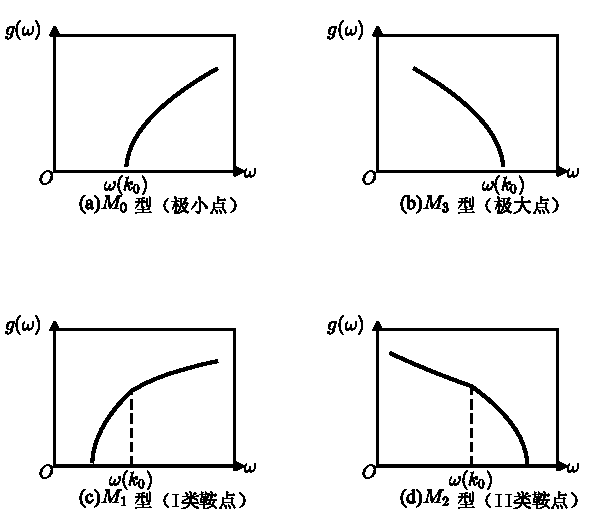
\includegraphics[width=10.5cm]{fig2-11.pdf}\\{\small 图 2.11\quad 范·霍夫奇点附近的态密度}
\end{minipage}
\end{center}

\section{晶格振动的局域模}

含有杂质和缺陷的晶体，由于平移对称性被破坏，其声子谱将不同于完整晶格，会产生以杂质、缺陷为中心的局域振动模式.

作为问题的第一步，我们将讨论单个杂质或缺陷对晶格振动谱的影响.从一维原子链入手，设质量为$M$的原子组成一维简单晶格，元胞数为$N$，在原点$(l=0)$处有一个质量为$M'$的杂质原子，近邻互作用的弹性力常数均设为$f$，如图2.12所示.因此
\begin{equation}
  M_1=\begin{cases}
  M&(l\neq0)\\
  M'&(l=0)
  \end{cases}
\end{equation}
并设
\begin{equation}
  \varepsilon\equiv\frac{M-M'}{M}
\end{equation}

\begin{center}
\begin{minipage}{9cm}
\centering
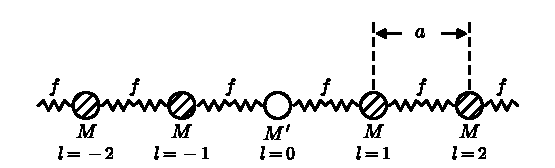
\includegraphics[width=9cm]{fig2-12.pdf}\\{\small 图 2.12\quad 含单个缺陷的一维链模型}
\end{minipage}
\end{center}

当$\varepsilon>0$时，代表“轻杂质”情况，而$\varepsilon<0$属于“重杂质”.由于杂质的存在，晶格振动的哈密顿量
\begin{equation}
  H=T+V
\end{equation}
其中动能部分
\begin{equation}
  T=\frac{1}{2}M\sum_l\dot{u}_l^2
  +\frac{1}{2}\bigl(M'-M\bigr)\dot{u}_{l=0}^2
\end{equation}
在简谐近似下根据图2.12规定的模型，其位能部分可简单写为
\begin{equation}
  V=\frac{1}{2}f\sum_l\bigl(u_l-u_{l+1}\bigr)^2
\end{equation}
$u_l$代表$l$元胞中原子的位移.下面将分别讨论式(2.10.3)的频谱及振动模特征.

\subsection*{1. 单个缺陷对振动频率的影响}

由于缺陷的存在，平移对称性被破坏，我们不能直接利用布洛赫定理来确定系统的振动模式，但可以利用傅里叶变换使求解简化，根据式(1.5.12)，晶格振动位移可表示为
\begin{equation}
  u_l=\frac{1}{\sqrt{N}}\sum_k\xi_k\mathrm{e}^{-\mathrm{i}kla}
\end{equation}
其中$k$限于BZ.将式(2.10.6)代入式(2.10.4)和式(2.10.5)，并利用关系式
\begin{equation}
  \frac{1}{N}\sum_l\mathrm{e}^{-\mathrm{i}(k+k')la}=\delta_{k',-k}
\end{equation}
可将$T$、$V$改用$\xi_k$、$\dot{\xi}_k$表示
\begin{equation}
\left.\begin{aligned}
  &T=\frac{1}{2}M\sum_k\dot{\xi}_k\dot{\xi}_{-k}
  +\frac{M'-M}{2N}\Bigl[\sum_k\dot{\xi}_k\Bigr]^2\\
  &V=\frac{1}{2}M\sum_k\omega_k^2\xi_k\xi_{-k}
\end{aligned}\right\}
\end{equation}
其中
\begin{equation}
  \omega_k^2=\omega_{\mathrm{M}}^2\sin^2\frac{ka}{2}
  \quad\left(\omega_{\mathrm{M}}^2=\frac{4f}{M}\right)
\end{equation}
代表完整晶格的本征振动频率，是$k$波矢格波的频率，属于平面波型解或称简正模.由于$M'$出现系统的本征频将发生改变，根据经典力学含缺陷系统的运动方程变为
\begin{equation}
  M\ddot{\xi}_k+\frac{M'-M}{N}\sum_k\ddot{\xi}_k
  =-M\omega_k^2\xi_k
\end{equation}
设$\xi_k\sim\exp(-\mathrm{i}\omega t)$，并利用式(2.10.2)将上式改写成
\begin{equation}
  \omega^2\Bigl(\xi_k-\frac{\varepsilon}{N}\sum_k\xi_k\Bigr)
  =\omega_k^2\xi_k
\end{equation}
考虑$\xi_k$的非零解，设
\begin{equation}
  \xi=\frac{1}{N}\sum_k\xi_k
\end{equation}
求得
\begin{equation}
  \xi_k=\varepsilon\,\frac{\xi\omega^2}{\bigl(\omega^2-\omega_k^2\bigr)}
\end{equation}
上式对$k$求和，再利用式(2.10.12)并消去$\xi$，得到确定含缺陷系统本征频率的方程为
\begin{equation}
  1=\frac{\varepsilon\omega^2}{N}\sum_k
  \frac{1}{\omega^2-\omega_k^2}\equiv F\bigl(\omega^2\bigr)
\end{equation}
式(2.10.14)可用作图法求解.图2.13(a)、(b)分别表示
$\varepsilon<0\,(M'>M$，重杂质$)$和$\varepsilon>0\,(M'<M$，轻杂质$)$情况.完整晶格的简正模频率$\omega_k$限于$0\to\omega_{\mathrm{M}}$区间，由图中黑点“$\bullet$”表示，图中“$\blacktriangle$”号代表含缺陷晶格的本征频率，它们满足式(2.10.14).显然，$F$函数是$\omega$的偶函数，在这里只画出了$\omega>0$部分，因为简单晶格的声频支解的最低频率为$\omega=0$.

由图2.13(a)可知，对于“重杂质”情况$(\varepsilon<0)$，式(2.10.14)的解仍落于声频支许可频带之内，非完整晶格的解(“$\blacktriangle$”)与完整晶格的简正模解(“$\bullet$”)有一一对应关系.由于杂质原子质量$M'$大于基体原子质量$M$，所有的解都向低频方向略有移动，其移动大小不超过两个近邻$\omega_k$值之差.又因为声频支频带下限在$\omega=0$处，这里没有单独的模式被推出频带底部.图中$\omega=0$模式解不明显出现，只是由于作图时所选用函数$F(\omega^2)$在$\omega=0$处无定义的缘故.

在图2.13(b)中$0<\varepsilon<1$，属于“轻杂质”情况.当$\omega<\omega_{\mathrm{M}}$时，式(2.10.14)的解相对于$\omega_k$都朝高频方向略有移动，在这里非完整晶格的解比$\omega_k$解少一个.这个解的移动较大，它被推出准连续频带顶部$(\omega_{\mathrm{M}})$，落在$\omega>\omega_{\mathrm{M}}$区域中，形成一个孤立的能级.通过下面的分析将明白，$\varepsilon>0$情况下$\omega>\omega_{\mathrm{M}}$的孤立解代表以杂质原子为中心的局域振动模式.

\begin{center}
\begin{minipage}{9.5cm}
\centering
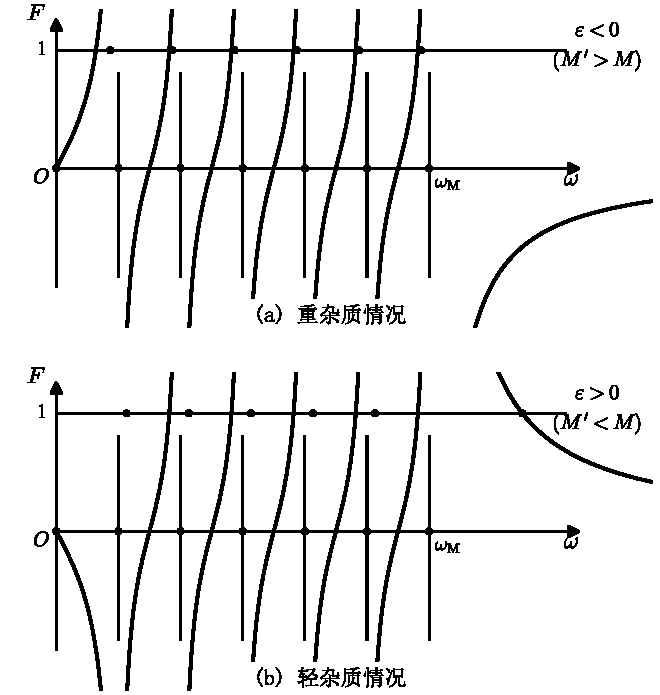
\includegraphics[width=9.5cm]{fig2-13.pdf}\\{\small 图 2.13\quad 式(2.10.14)的作图解}
\end{minipage}
\end{center}

\subsection*{2. 局域模\textsuperscript{[6]}}

为了分析振动模式，必须解$u_l$的运动方程.根据式(2.10.4)、(2.10.5)和(2.10.2)容易写出运动方程
\begin{equation}
  M\ddot{u}_l-f\bigl(u_{l+1}+u_{l-1}-2u_l\bigr)
  =\varepsilon M\ddot{u}_0\delta_{l0}
\end{equation}
其中$\delta_{l0}$为克罗尼克(Kr\"onecker)$\delta$函数.令$u_l\sim\exp(-\mathrm{i}\omega t)$.将上式写为
\begin{equation}
  u_1+u_{-1}
  +\biggl[\frac{4\omega^2}{\omega_{\mathrm{M}}^2}(1-\varepsilon)-2\biggr]u_0=0
\end{equation}
和
\begin{equation}
  u_{l+1}+u_{l-1}
  +\left(\frac{4\omega^2}{\omega_{\mathrm{M}}^2}-2\right)u_l=0
  \quad(l\neq0)
\end{equation}
其中$\omega_{\mathrm{M}}^2=\frac{4f}{M}$.振动的特征应由式(2.10.16)与(2.10.17)的联立解确定.由于杂质位于$l=0$点，这里存在着对称解$(u_l=u_{-l})$和反对称解$(u_l=-u_{-l})$.反对称解要求$u_0=0$和$u_l+u_{-l}=0$，因此式(2.10.16)不起作用，可不讨论.下面仅研究对称解，可设解的一般形式为
\begin{equation}
  u_l=A\lambda^{|l|}+B\lambda^{-|l|}
\end{equation}
代入式(2.10.17)得到
\begin{equation}
  \lambda^2+1+\left(\frac{4\omega^2}{\omega_{\mathrm{M}}^2}-2\right)\lambda=0
\end{equation}
由式(2.10.19)可以判断$\lambda$根的性质.当$\omega<\omega_{\mathrm{M}}$时，方程有复根，可设$\lambda$为$\exp(\mathrm{i}\theta)$形式并取$\theta=ka$，属于格波解.当$\omega>\omega_{\mathrm{M}}$时$\lambda$有负实根，其中一个$|\lambda|<1$、另一个$|\lambda|>1$，这时将求得局域晶格振动解.下面分别讨论：

(i)对于$\omega<\omega_{\mathrm{M}}$情况：可令
\begin{equation}
  u_l=A\exp(\mathrm{i}ka|l|)+B\exp(-\mathrm{i}ka|l|)
\end{equation}
代入式(2.10.16)得到方程
\begin{equation}
  \frac{A\exp(\mathrm{i}ka)+B\exp(-\mathrm{i}ka)}{A+B}
  +\biggl[\frac{2\omega^2}{\omega_{\mathrm{M}}^2}(1-\varepsilon)-1\biggr]=0
\end{equation}
考虑到$u_l$为实量，应有$A^{*}=B$关系.因此，可进一步假定
\begin{equation}
  A=\frac{c}{2}\exp(-\mathrm{i}\delta)\,,\quad
  B=\frac{c}{2}\exp(\mathrm{i}\delta)
\end{equation}
代入式(2.10.20)和式(2.10.21)求得在$0<\omega<\omega_{\mathrm{M}}$频带内的解
\begin{equation}
  u_l=c\cos\bigl(|l|ka-\delta\bigr)
\end{equation}
其中$\delta$代表相移，它满足方程
\begin{equation}
  \tan\delta=\varepsilon\tan\frac{ka}{2}
\end{equation}
以上结果说明，杂质的存在仅使简正模产生相移，相移的正负取决于$\varepsilon$的符号，这是和图2.13(a)及(b)中，$\omega<\omega_{\mathrm{M}}$时本征频率的微小移动相对应的.

(ii)对于$\omega>\omega_{\mathrm{M}}$的情况：讨论$|\lambda|<1$情况的负实根，这时可设对称解为
\begin{equation}
  u_l=A\lambda^{|l|}
\end{equation}
代入式(2.10.16)和式(2.10.17)得到方程组
\begin{equation}
\begin{gathered}
  2\lambda+\biggl[\frac{4\omega^2}{\omega_{\mathrm{M}}^2}(1-\varepsilon)-2\biggr]=0\\[1ex]
  \lambda^2+1+\left(\frac{4\omega^2}{\omega_{\mathrm{M}}^2}-2\right)\lambda=0
\end{gathered}
\end{equation}
联立求解可得
\begin{equation}
  (\lambda-1)\biggl[2-\frac{\lambda-1}{\lambda}(1-\varepsilon)\biggr]=0
\end{equation}
由于$\lambda\neq1$，因此$|\lambda|<1$的负根为
\begin{equation}
  \lambda=\frac{\varepsilon-1}{\varepsilon+1}
\end{equation}
其中$\varepsilon>0$，属于“轻杂质”情况.

将此解代入式(2.10.25)和式(2.10.26)第二个方程，给出位移
\begin{equation}
  u_l=u_0(-1)^l
  \left(\frac{1-\varepsilon}{1+\varepsilon}\right)^{|l|}
  \quad(\varepsilon>0)
\end{equation}
其振动频率
\begin{equation}
  \omega^2=\frac{\omega_{\mathrm{M}}^2}{1-\varepsilon}
\end{equation}
式(2.10.29)是以杂质为中心的衰减振荡解，其中近邻原子振动的方向相反，这就是晶格振动的局域模，其振动频率在$\omega_{\mathrm{M}}$之上，即图2.13(b)中的孤立能级，说明“轻杂质”将在声频支许可频带之上产生局域模.

局域模相当于$\lambda$取复数波矢$k$的解.若令
\begin{equation}
\left.\begin{aligned}
  &ka=\theta=\pi+\mathrm{i}Z\\
  &Z=\ln\left(\frac{1-\varepsilon}{1+\varepsilon}\right)
\end{aligned}\right\}
\end{equation}
则得到式(2.10.28)的结果
\begin{equation}
  \lambda=\mathrm{e}^{-\mathrm{i}ka}=\frac{\varepsilon-1}{\varepsilon+1}
\end{equation}
因此局域模又可写成下列指数形式
\begin{equation}
  u_l=u_0\mathrm{e}^{\mathrm{i}ka|l|}
\end{equation}
其中
\begin{equation}
  k=\frac{\pi}{a}+\mathrm{i}\frac{Z}{a}
\end{equation}
在一维链中的单个点缺陷(空位)与单杂质情况相似，这时$M'=0$，点缺陷的近邻常数应设为$f'$(与$f$不同).增大或减小单个力常数分别与减少或增大单个杂质原子的质量有相同的效应，读者可仿效以上做法自行处理点缺陷的局域模问题.

最后指出本节主要结论是：

(i)“轻杂质”将使简正模频率向上推移，并在许可频带之上分裂出一个局域模.增大杂质与基体原子的质量差$(\varepsilon)$，局域频率与许可频带上边界的距离也就拉得越开[见式(2.10.30)].

(ii)“重杂质”的效应是使本征频率向下移动，对于声频支振动许可频带的下界在$\omega=0$处，因此不可能在下界之外分裂出局域模.但是对于光频支振动，其许可频带的下界为非零值，在这种情况下“重杂质”就可能在频带之下产生一个分立能级——局域模.

\begin{canKao}
\begin{enumerate}[label={[\arabic*]}, leftmargin=2.2em, itemsep=0pt]
\item Born M, Huang K. Dynamical Theory of Crystal Lattice. Oxford: Clarenden Press, 1954
\item van Hove L. Phys Rev, 1953, 89: 1189
\item Wannier G H. Elements of Solid State Theory. London: Cambridge Univ Press, 1959
\item Callaway J. Quantum Theory of Solid State. New York: Academic Press, 1976
\item Maradudin A A. Solid State Phys. Suppl. 3 (2nd ed). New York: Academic Press, 1971
\item Madelung O. Introduction to Solid State Theory. New York: Springer Press, 1980. Chap9
\end{enumerate}
\end{canKao}
